% Options for packages loaded elsewhere
% Options for packages loaded elsewhere
\PassOptionsToPackage{unicode}{hyperref}
\PassOptionsToPackage{hyphens}{url}
\PassOptionsToPackage{dvipsnames,svgnames,x11names}{xcolor}
%
\documentclass[
  11pt,
]{article}
\usepackage{xcolor}
\usepackage[lmargin=1in,rmargin=1in,tmargin=1in,bmargin=1in]{geometry}
\usepackage{amsmath,amssymb}
\setcounter{secnumdepth}{-\maxdimen} % remove section numbering
\usepackage{iftex}
\ifPDFTeX
  \usepackage[T1]{fontenc}
  \usepackage[utf8]{inputenc}
  \usepackage{textcomp} % provide euro and other symbols
\else % if luatex or xetex
  \usepackage{unicode-math} % this also loads fontspec
  \defaultfontfeatures{Scale=MatchLowercase}
  \defaultfontfeatures[\rmfamily]{Ligatures=TeX,Scale=1}
\fi
\usepackage{lmodern}
\ifPDFTeX\else
  % xetex/luatex font selection
\fi
% Use upquote if available, for straight quotes in verbatim environments
\IfFileExists{upquote.sty}{\usepackage{upquote}}{}
\IfFileExists{microtype.sty}{% use microtype if available
  \usepackage[]{microtype}
  \UseMicrotypeSet[protrusion]{basicmath} % disable protrusion for tt fonts
}{}
\makeatletter
\@ifundefined{KOMAClassName}{% if non-KOMA class
  \IfFileExists{parskip.sty}{%
    \usepackage{parskip}
  }{% else
    \setlength{\parindent}{0pt}
    \setlength{\parskip}{6pt plus 2pt minus 1pt}}
}{% if KOMA class
  \KOMAoptions{parskip=half}}
\makeatother
% Make \paragraph and \subparagraph free-standing
\makeatletter
\ifx\paragraph\undefined\else
  \let\oldparagraph\paragraph
  \renewcommand{\paragraph}{
    \@ifstar
      \xxxParagraphStar
      \xxxParagraphNoStar
  }
  \newcommand{\xxxParagraphStar}[1]{\oldparagraph*{#1}\mbox{}}
  \newcommand{\xxxParagraphNoStar}[1]{\oldparagraph{#1}\mbox{}}
\fi
\ifx\subparagraph\undefined\else
  \let\oldsubparagraph\subparagraph
  \renewcommand{\subparagraph}{
    \@ifstar
      \xxxSubParagraphStar
      \xxxSubParagraphNoStar
  }
  \newcommand{\xxxSubParagraphStar}[1]{\oldsubparagraph*{#1}\mbox{}}
  \newcommand{\xxxSubParagraphNoStar}[1]{\oldsubparagraph{#1}\mbox{}}
\fi
\makeatother


\usepackage{longtable,booktabs,array}
\usepackage{calc} % for calculating minipage widths
% Correct order of tables after \paragraph or \subparagraph
\usepackage{etoolbox}
\makeatletter
\patchcmd\longtable{\par}{\if@noskipsec\mbox{}\fi\par}{}{}
\makeatother
% Allow footnotes in longtable head/foot
\IfFileExists{footnotehyper.sty}{\usepackage{footnotehyper}}{\usepackage{footnote}}
\makesavenoteenv{longtable}
\usepackage{graphicx}
\makeatletter
\newsavebox\pandoc@box
\newcommand*\pandocbounded[1]{% scales image to fit in text height/width
  \sbox\pandoc@box{#1}%
  \Gscale@div\@tempa{\textheight}{\dimexpr\ht\pandoc@box+\dp\pandoc@box\relax}%
  \Gscale@div\@tempb{\linewidth}{\wd\pandoc@box}%
  \ifdim\@tempb\p@<\@tempa\p@\let\@tempa\@tempb\fi% select the smaller of both
  \ifdim\@tempa\p@<\p@\scalebox{\@tempa}{\usebox\pandoc@box}%
  \else\usebox{\pandoc@box}%
  \fi%
}
% Set default figure placement to htbp
\def\fps@figure{htbp}
\makeatother





\setlength{\emergencystretch}{3em} % prevent overfull lines

\providecommand{\tightlist}{%
  \setlength{\itemsep}{0pt}\setlength{\parskip}{0pt}}



 


\makeatletter
\@ifpackageloaded{caption}{}{\usepackage{caption}}
\AtBeginDocument{%
\ifdefined\contentsname
  \renewcommand*\contentsname{Table of contents}
\else
  \newcommand\contentsname{Table of contents}
\fi
\ifdefined\listfigurename
  \renewcommand*\listfigurename{List of Figures}
\else
  \newcommand\listfigurename{List of Figures}
\fi
\ifdefined\listtablename
  \renewcommand*\listtablename{List of Tables}
\else
  \newcommand\listtablename{List of Tables}
\fi
\ifdefined\figurename
  \renewcommand*\figurename{Figure}
\else
  \newcommand\figurename{Figure}
\fi
\ifdefined\tablename
  \renewcommand*\tablename{Table}
\else
  \newcommand\tablename{Table}
\fi
}
\@ifpackageloaded{float}{}{\usepackage{float}}
\floatstyle{ruled}
\@ifundefined{c@chapter}{\newfloat{codelisting}{h}{lop}}{\newfloat{codelisting}{h}{lop}[chapter]}
\floatname{codelisting}{Listing}
\newcommand*\listoflistings{\listof{codelisting}{List of Listings}}
\makeatother
\makeatletter
\makeatother
\makeatletter
\@ifpackageloaded{caption}{}{\usepackage{caption}}
\@ifpackageloaded{subcaption}{}{\usepackage{subcaption}}
\makeatother
\usepackage{bookmark}
\IfFileExists{xurl.sty}{\usepackage{xurl}}{} % add URL line breaks if available
\urlstyle{same}
\hypersetup{
  pdftitle={Gender Gaps in Education: A Cross-Regional Analysis of Enrollment and Teacher Quality},
  pdfauthor={Ayushi Chowksey (2556332); Hank Standaert (2558027); Ryana Rajesh (2549737); Chau Anh Nguyen (2575963); Jacob Hillman (2580176)},
  colorlinks=true,
  linkcolor={blue},
  filecolor={Maroon},
  citecolor={Blue},
  urlcolor={Blue},
  pdfcreator={LaTeX via pandoc}}


\title{Gender Gaps in Education: A Cross-Regional Analysis of Enrollment
and Teacher Quality}
\usepackage{etoolbox}
\makeatletter
\providecommand{\subtitle}[1]{% add subtitle to \maketitle
  \apptocmd{\@title}{\par {\large #1 \par}}{}{}
}
\makeatother
\subtitle{DATASCI 350 - Final Project}
\author{Ayushi Chowksey (2556332) \and Hank Standaert
(2558027) \and Ryana Rajesh (2549737) \and Chau Anh Nguyen
(2575963) \and Jacob Hillman (2580176)}
\date{2026-04-27}
\begin{document}
\maketitle


\section{Introduction}\label{introduction}

Introduction This project examines global education patterns using data
from the World Bank's World Development Indicators (WDI), with a focus
on school enrollment across primary, secondary, and tertiary levels. The
WDI EdStats Query holds around 2,500 internationally comparable
education indicators covering access, progression, completion, literacy,
teachers, population, and expenditures (World Bank, ``Education
Statistics''). Rather than analyzing individual countries, the study
compares aggregated regional and income-based groupings provided by the
World Bank, allowing for a broader and more structured analysis of
global education systems. The analysis includes gender-disaggregated
enrollment data and measures of trained teachers to provide a
multidimensional view of education.

Education is a key driver of economic development, human capital
formation, and long-term growth. Research confirms the positive effects
of enrollment rates, average years of schooling, education spending, and
education quality on economic growth (Wang et al.). While enrollment
rates provide an important measure of access to schooling, they do not
fully capture the effectiveness or equity of education systems. Gender
differences in enrollment can reveal persistent inequalities in access,
while the proportion of trained teachers reflects the quality of
education systems. Teacher quality has long been acknowledged as a
crucial educational input and a predictor of instructional quality,
which in turn leads to better student achievement (Pholphirul).
Examining these factors across both regional and income-based groupings
allows for a more systematic understanding of how development levels
relate to enrollment.

This analysis is guided by two primary research questions. First, how do
male and female enrollment rates differ across global regions and income
groups from 2000 to 2023, and how do these differences vary across
levels of education? Second, how does the proportion of trained teachers
in secondary education relate to enrollment levels across these
groupings?

To address these questions, we construct a dataset from multiple WDI
education indicators and apply a series of data cleaning and
preprocessing steps to ensure consistency across regions, income groups,
and years.

\section{Data Description}\label{data-description}

The dataset used in this project is drawn from the World Bank's World
Development Indicators (WDI), which contains over 1,600 indicators
across more than 200 countries and territories from 1960 to 2023. In
addition to country-level data, the WDI provides pre-aggregated
indicators for regional groupings (e.g., East Asia \& Pacific, Europe \&
Central Asia) and income-based groupings. This project focuses on these
aggregated regional and income categories rather than individual
countries.

The analysis uses a subset of education-related indicators, including
school enrollment rates at the primary, secondary, and tertiary levels,
gender-disaggregated enrollment measures, and the proportion of trained
teachers. These indicators are selected to capture key dimensions of
education systems, including access to schooling, equity across gender,
and the quality of instruction.

To ensure consistency and comparability, the dataset is restricted to
selected regional and income groupings and to the time period from 2000
to 2023.

\subsection{Regions and Income Groups}\label{regions-and-income-groups}

The following 13 regional and income groupings are included in the
analysis:

\begin{longtable}[]{@{}ll@{}}
\toprule\noalign{}
Region / Group & Code \\
\midrule\noalign{}
\endhead
\bottomrule\noalign{}
\endlastfoot
Africa Eastern \& Southern & AFE \\
Africa Western \& Central & AFW \\
Arab World & ARB \\
Australia & AUS \\
East Asia \& Pacific & EAS \\
European Union & EUU \\
Latin America \& Caribbean & LCN \\
North America & NAC \\
South Asia & SAS \\
Low income & LIC \\
Lower middle income & LMC \\
Upper middle income & UMC \\
High income & HIC \\
\end{longtable}

\subsection{Data Cleaning --- Enrollment
Data}\label{data-cleaning-enrollment-data}

Enrollment data for primary, secondary, and tertiary levels was
downloaded separately for male and female students from the World Bank
WDI database. Each file was loaded into Python, filtered to include only
the 13 target region/income codes and years 2000--2023, and reshaped
from wide format into long format using SQL via SQLite in Python. Male
and female tables were then merged on \texttt{country\_code} and
\texttt{year} to produce a single merged dataset for each education
level. The process was repeated identically for primary, secondary, and
tertiary enrollment.

\subsection{Data Cleaning --- Trained Teacher
Data}\label{data-cleaning-trained-teacher-data}

After assessing the structure of the dataset and the extent of missing
values, the data was restricted to observations from 2000 to 2023 and to
the selected regional and income-group country codes. The preliminary
data file was in wide format and was reshaped into long format with the
variables country\_name, country\_code, year, and trained\_teacher using
SQLite in Python. The final cleaned file contained 312 country-year
observations, of which only 126 had non-missing values for
trained\_teacher.

\begin{figure}

\begin{minipage}{0.50\linewidth}

\begin{figure}[H]

{\centering 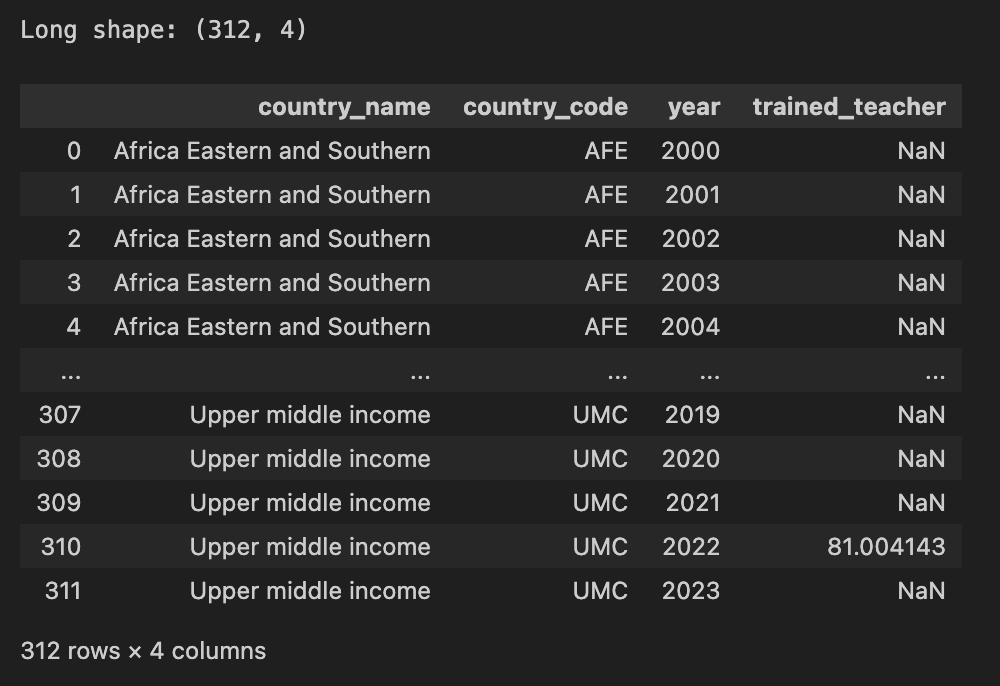
\includegraphics[width=0.95\linewidth,height=\textheight,keepaspectratio]{../figures/trained_teacher_trained_structure.png}

}

\subcaption{Dataset structure}

\end{figure}%

\end{minipage}%
%
\begin{minipage}{0.50\linewidth}

\begin{figure}[H]

{\centering 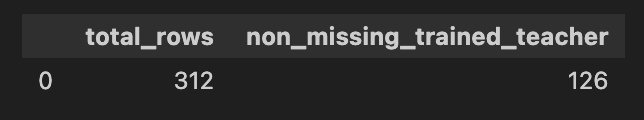
\includegraphics[width=0.95\linewidth,height=\textheight,keepaspectratio]{../figures/trained_teacher_missing.png}

}

\subcaption{Missing values summary}

\end{figure}%

\end{minipage}%

\end{figure}%

The histogram of trained teacher percentages shows a distribution
concentrated mostly between 55 and 100 percent, with heavier clustering
toward the upper end. The mean was 78.67 and the median was 80.43,
indicating a mild left skew. The time-series plot showed no clear linear
trend --- the yearly mean declined from the early 2000s into the early
2010s before recovering in later years. Interestingly, the median falls
below the mean in the late 2000s before rising above it around 2015,
reflecting a changing distribution of trained teacher percentages over
time.

\begin{figure}

\begin{minipage}{0.50\linewidth}

\begin{figure}[H]

{\centering 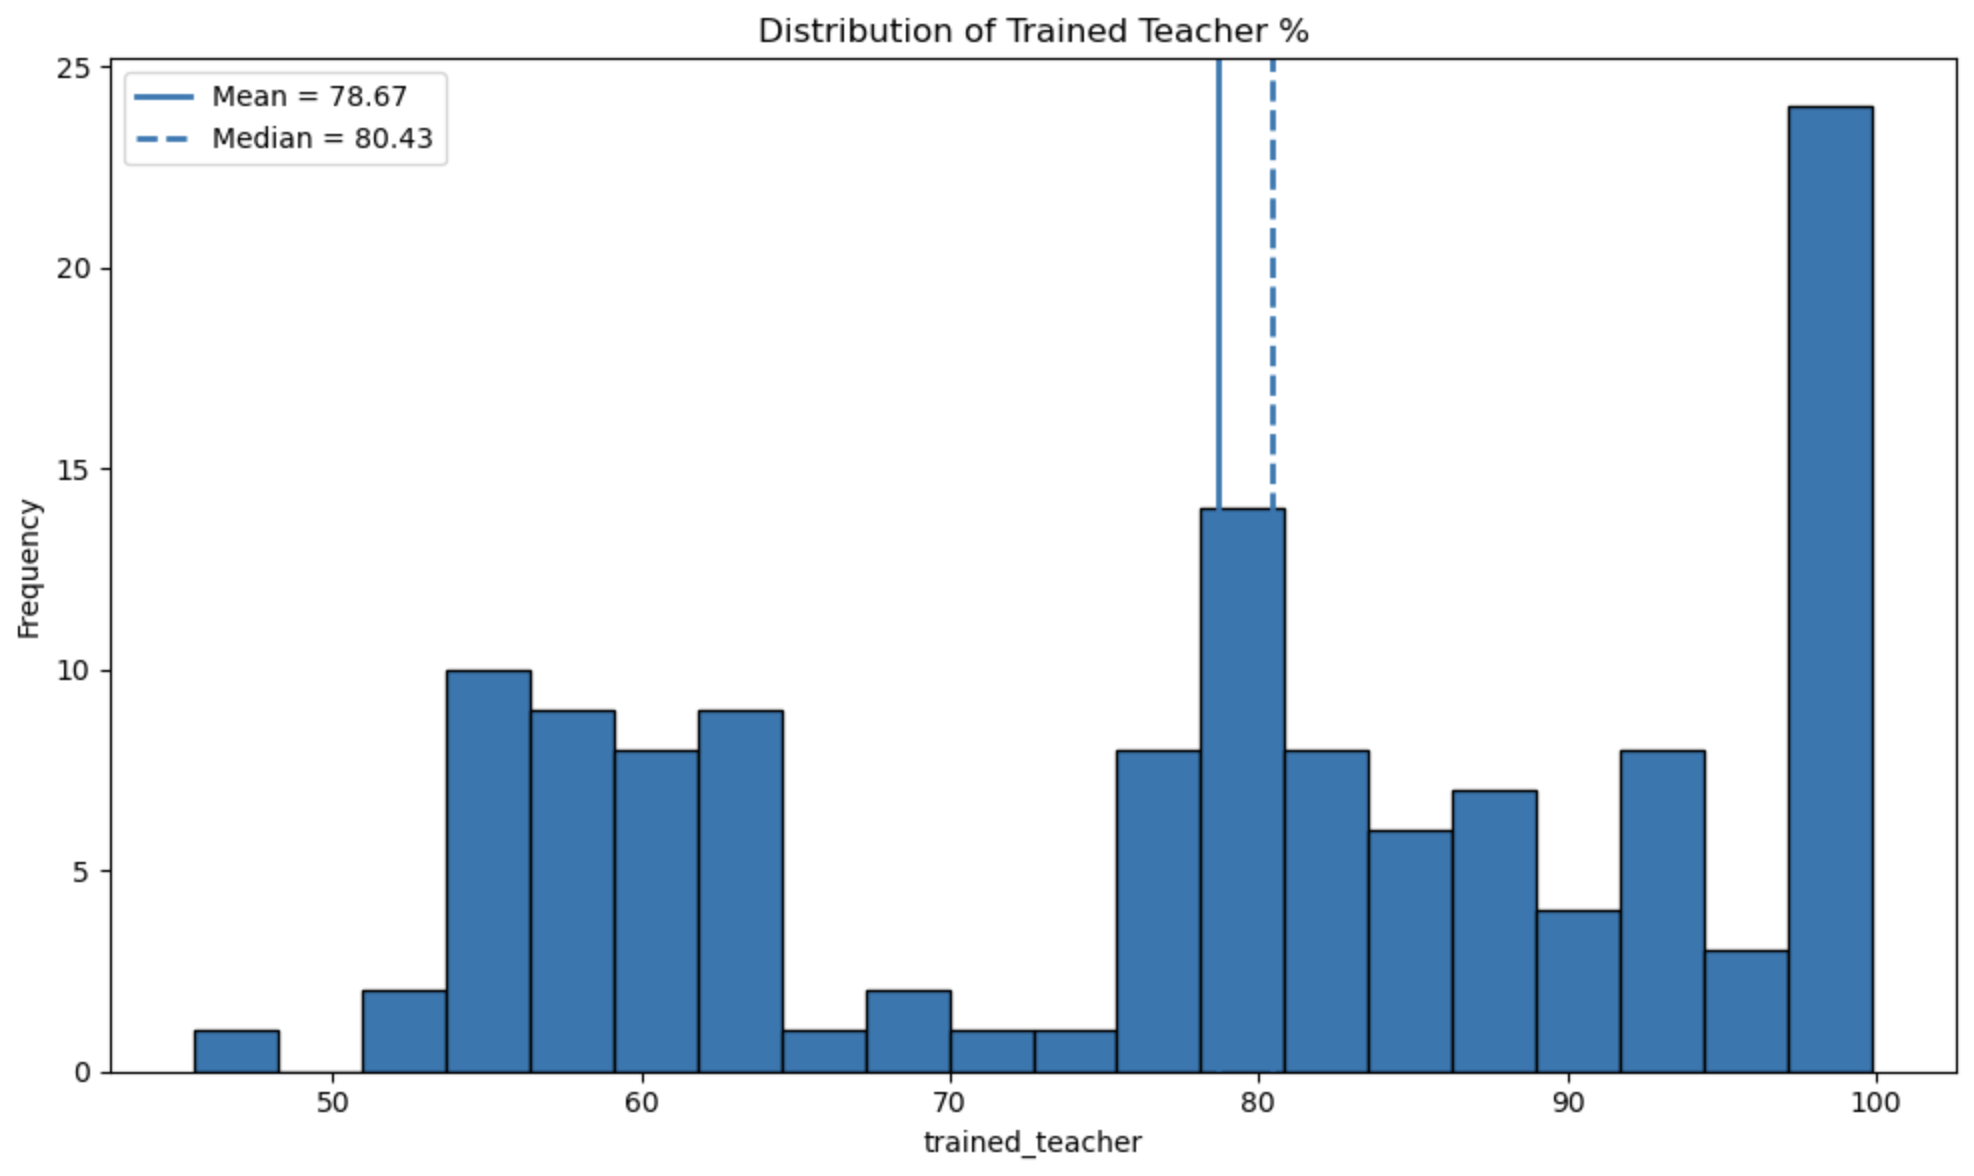
\includegraphics[width=0.95\linewidth,height=\textheight,keepaspectratio]{../figures/trained_teacher_histogram.png}

}

\subcaption{Trained teacher distribution}

\end{figure}%

\end{minipage}%
%
\begin{minipage}{0.50\linewidth}

\begin{figure}[H]

{\centering 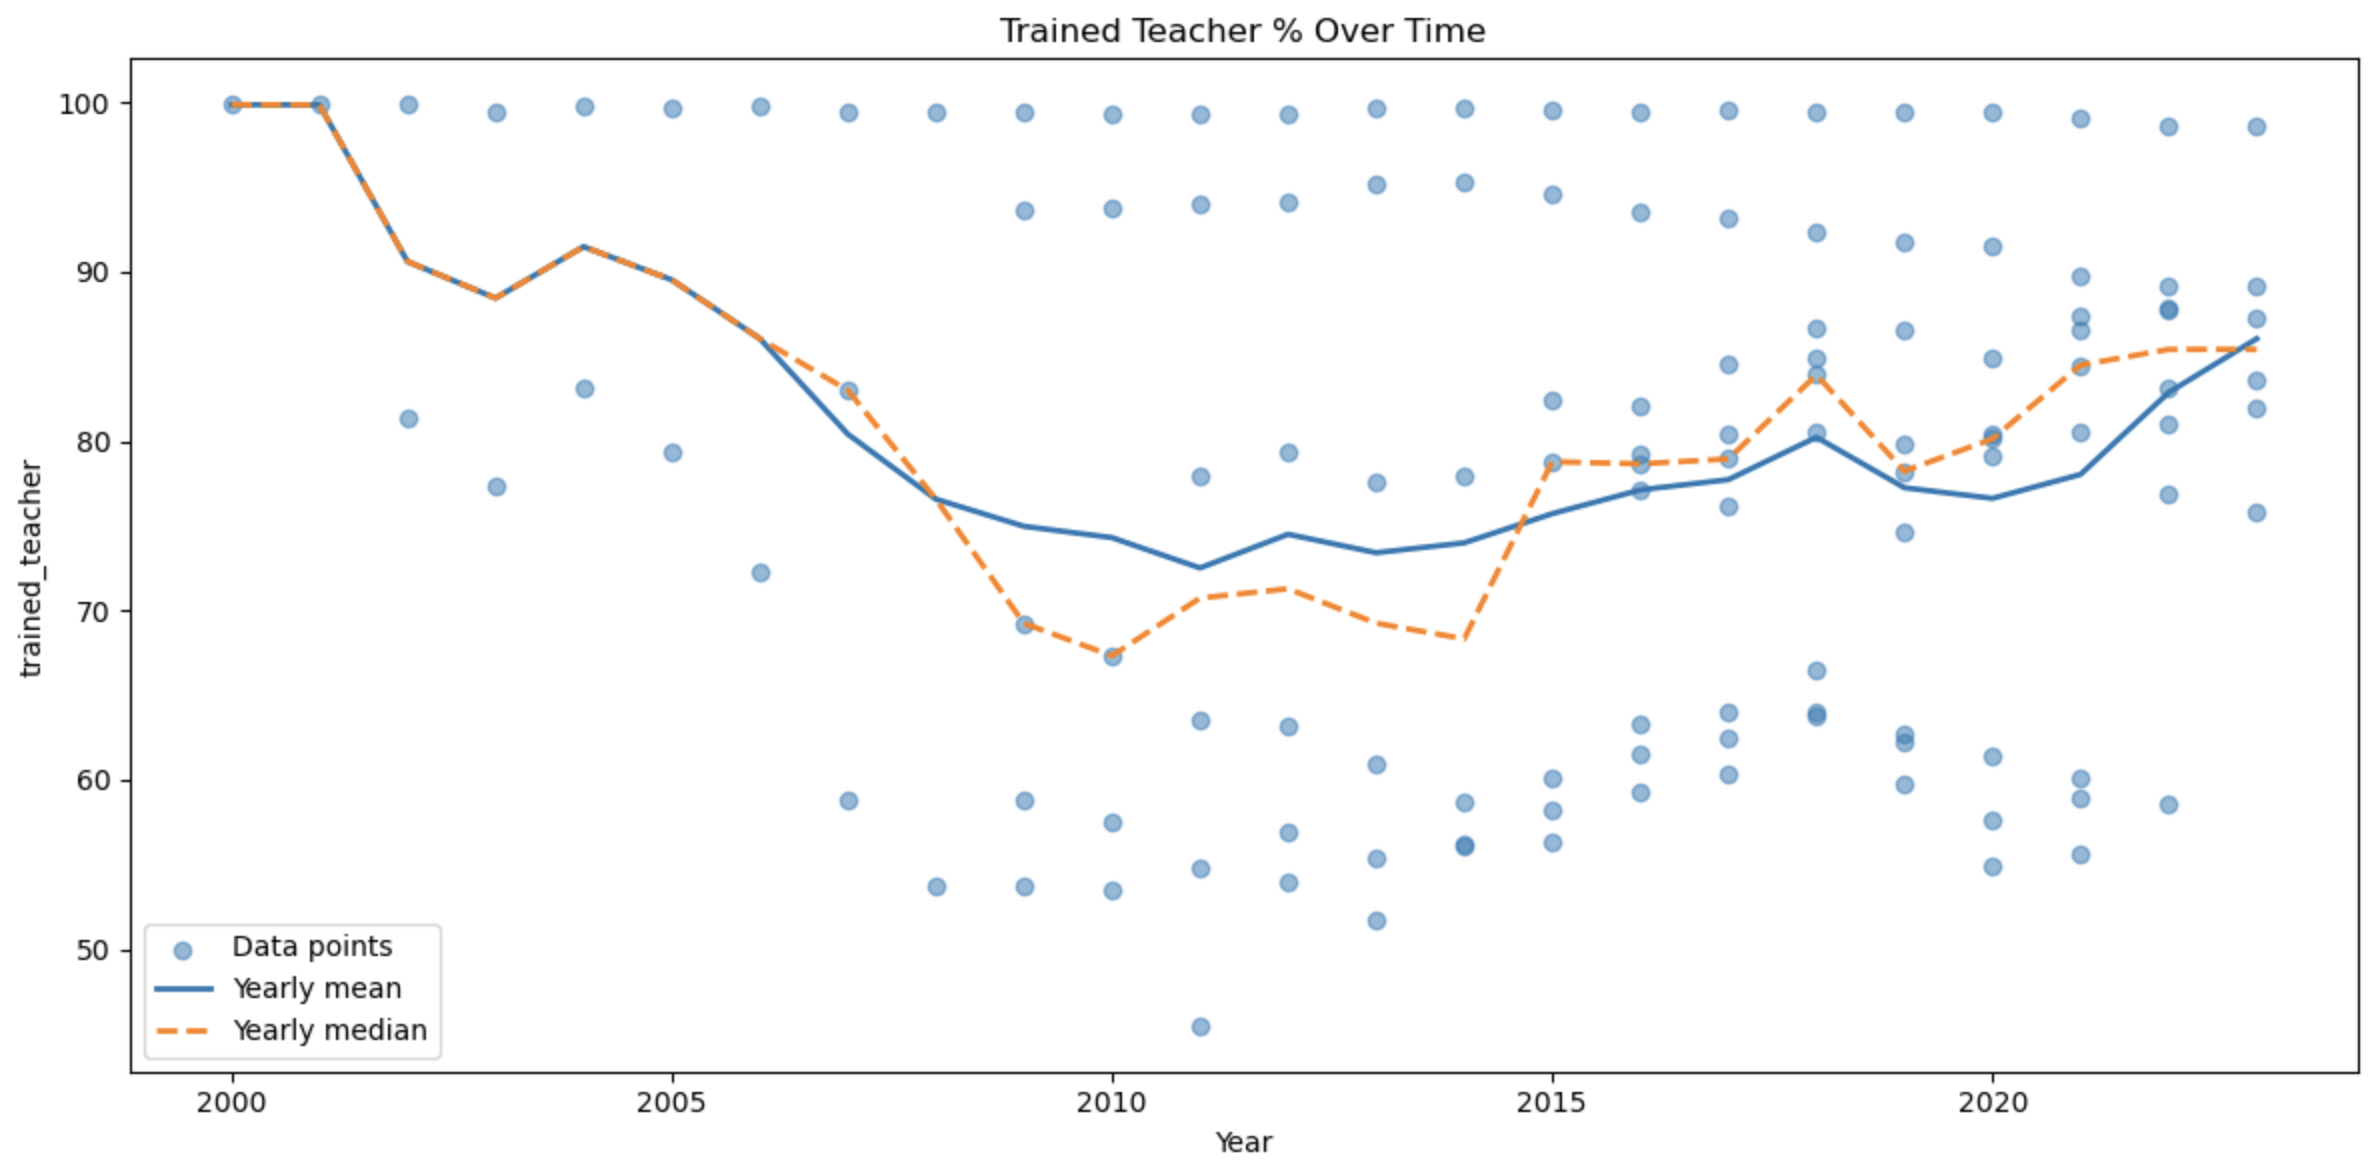
\includegraphics[width=0.95\linewidth,height=\textheight,keepaspectratio]{../figures/trained_teacher_trend.png}

}

\subcaption{Trained teacher over time}

\end{figure}%

\end{minipage}%

\end{figure}%

\section{Data Analysis}\label{data-analysis}

\subsection{SQL Exploratory Data
Analysis}\label{sql-exploratory-data-analysis}

Before conducting the full analysis, we used SQL queries via SQLite in
Python to compute descriptive statistics across all three education
levels combined.

The SQL queries reveal clear differences across education levels. At the
primary level, average male enrollment (101.45\%) slightly exceeds
female enrollment (98.45\%), producing a small average gender gap of
-3.01 percentage points (female minus male). At the secondary level,
average male enrollment (75.21\%) again slightly exceeds female
(72.99\%), with an average gap of -2.22 points. At the tertiary level,
the pattern reverses --- female enrollment (41.57\%) substantially
exceeds male enrollment (34.91\%), with an average gap of +6.65
percentage points in favor of females.

\subsubsection{Enrollment Percentage Change from 2000 to
2023}\label{enrollment-percentage-change-from-2000-to-2023}

We also computed the percentage change in male and female enrollment
from 2000 to 2023 for each region and education level using SQL.

At the primary level, the largest female enrollment gains occurred in
low-income regions --- Low income (LIC) saw a 54.01\% increase in female
enrollment compared to 29.87\% for males. Africa Eastern \& Southern
(AFE) saw a 34.71\% female increase versus 22.20\% for males, and Africa
Western \& Central (AFW) saw a 24.95\% female increase versus only
3.26\% for males. High-income regions saw small declines, consistent
with already near-universal enrollment.

At the secondary level, AFW saw a 145.51\% increase in female secondary
enrollment versus 81.01\% for males --- the fastest female growth of any
region. South Asia (SAS) saw a 93.69\% female increase versus 43.33\%
for males. High-income regions saw much smaller gains of around 2--5\%
for both genders.

At the tertiary level, growth was dramatic across all regions. Upper
middle income (UMC) saw female enrollment grow by 365.86\% compared to
273.87\% for males. South Asia saw female tertiary enrollment grow by
359.01\% versus 187.65\% for males. Even high-income regions saw
substantial female tertiary growth --- North America grew 27.16\% for
females versus 17.52\% for males. These results confirm that female
tertiary enrollment has been growing faster than male across virtually
every region.

\subsection{RQ1: Male vs.~Female Enrollment Across Regions and Education
Levels}\label{rq1-male-vs.-female-enrollment-across-regions-and-education-levels}

To address the first research question, we analyzed gender-disaggregated
enrollment rates across primary, secondary, and tertiary education from
2000 to 2023. A gender gap variable was computed as male enrollment
minus female enrollment, where positive values indicate higher male
enrollment and negative values indicate higher female enrollment.

\subsubsection{Primary Enrollment}\label{primary-enrollment}

At the primary level, male gross enrollment has consistently exceeded
female enrollment, though the gap has narrowed significantly. In 2000,
the gender gap was approximately 7 percentage points, with male
enrollment near 100\% and female enrollment around 93\%. The gap
declined steadily through 2016, reaching a low of about 0.6 percentage
points, before stabilizing at roughly 1.5 points by 2023.

\begin{figure}

\begin{minipage}{0.50\linewidth}

\begin{figure}[H]

{\centering 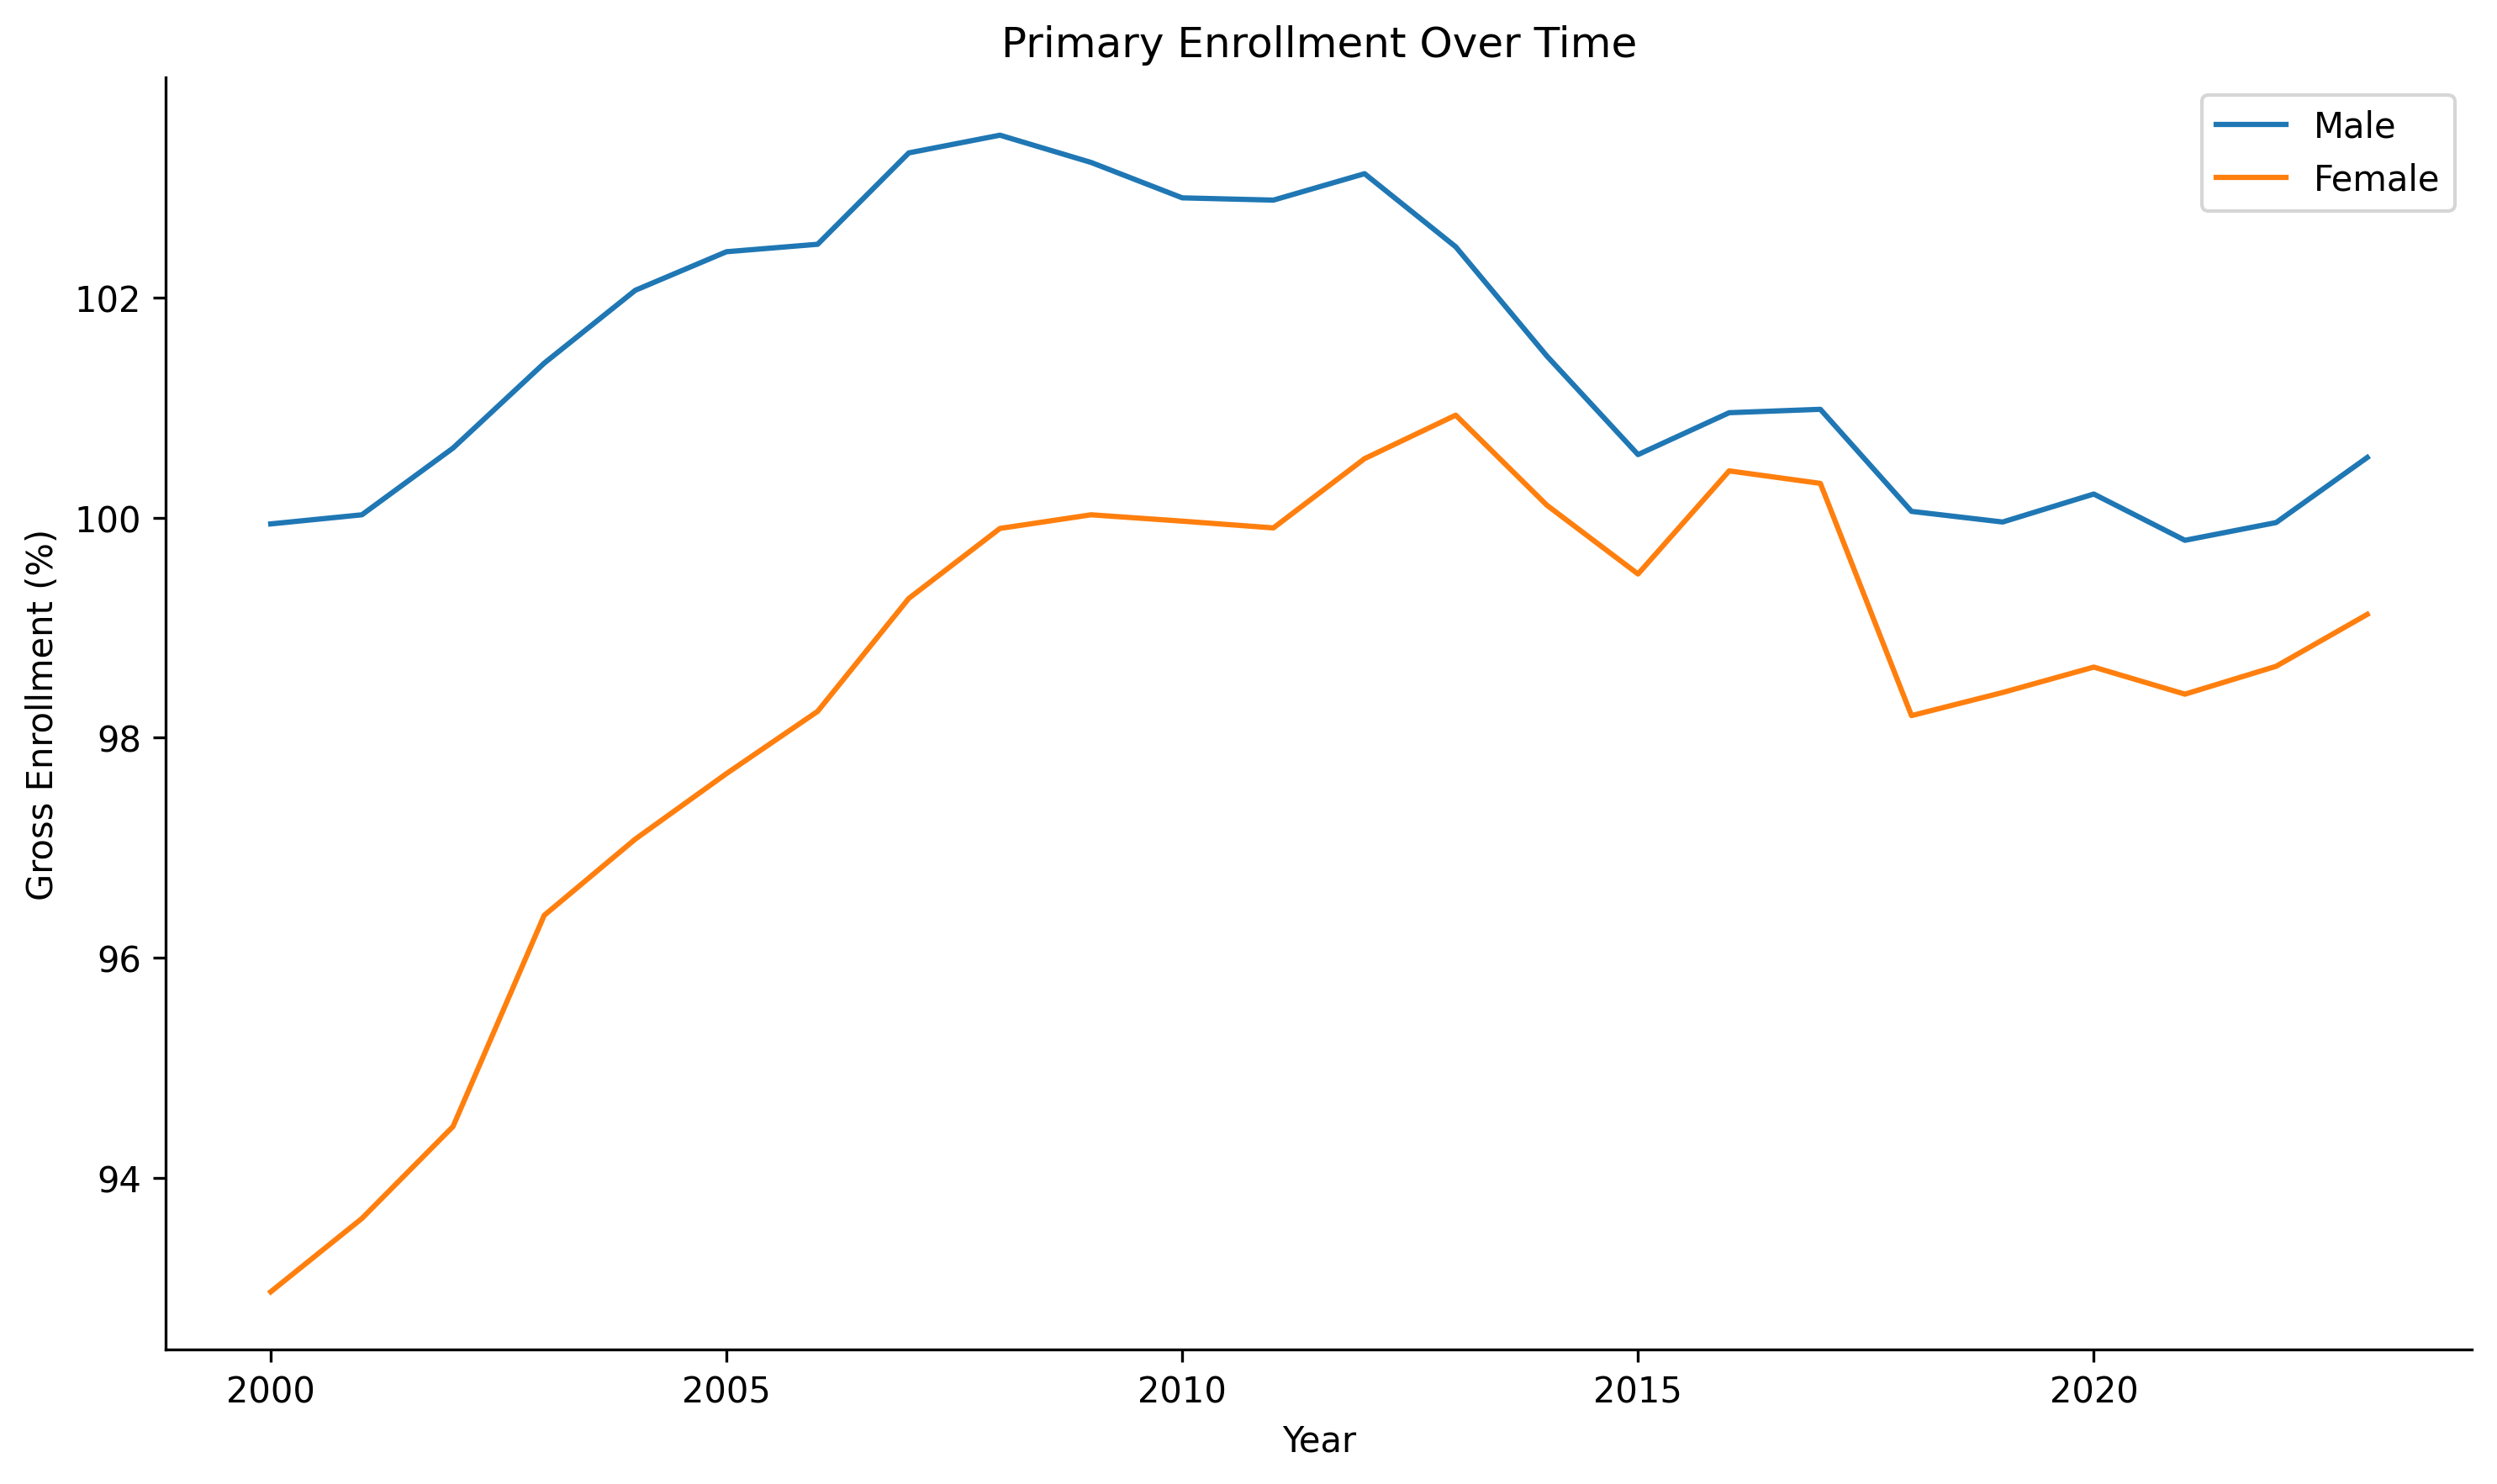
\includegraphics[width=0.95\linewidth,height=\textheight,keepaspectratio]{../figures/primary_gender_trends.png}

}

\subcaption{Primary school enrollment trends by gender (2000--2023)}

\end{figure}%

\end{minipage}%
%
\begin{minipage}{0.50\linewidth}

\begin{figure}[H]

{\centering 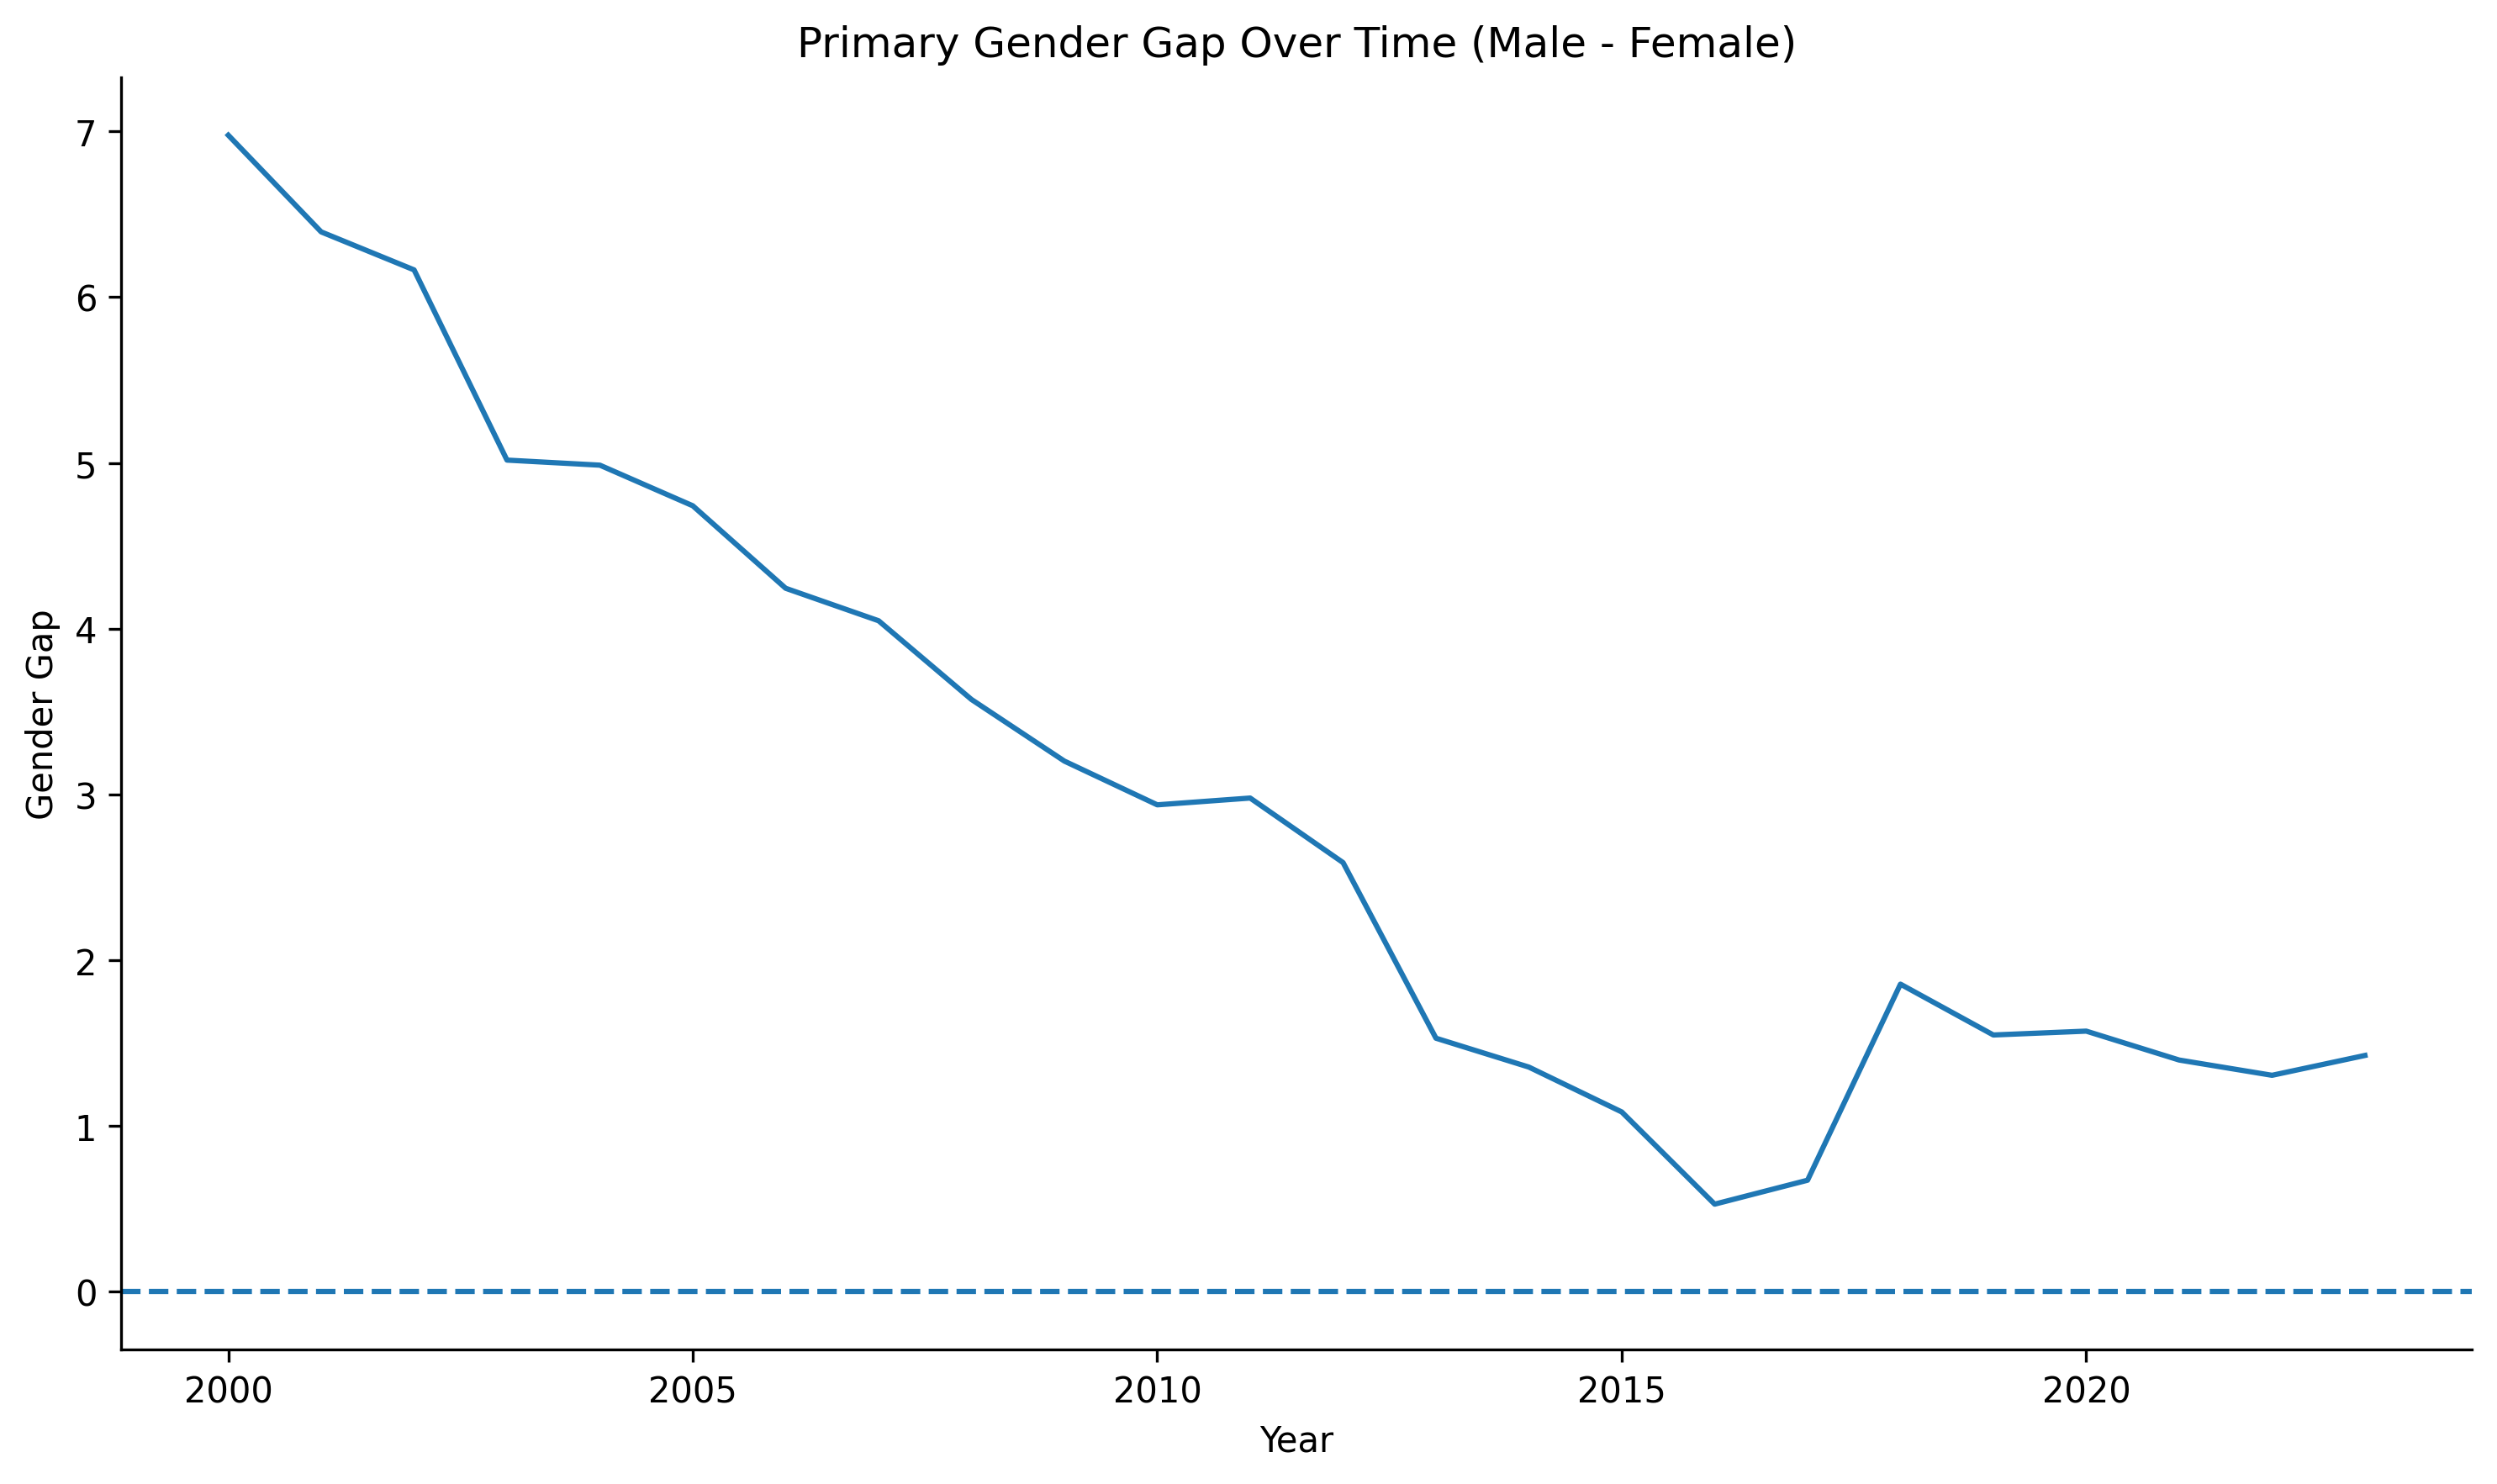
\includegraphics[width=0.95\linewidth,height=\textheight,keepaspectratio]{../figures/primary_gap_trend.png}

}

\subcaption{Gender gap in primary enrollment over time}

\end{figure}%

\end{minipage}%

\end{figure}%

\subsubsection{Secondary Enrollment}\label{secondary-enrollment}

Secondary enrollment shows strong growth for both genders. Male
enrollment rose from approximately 63\% in 2000 to around 83\% by 2023,
while female enrollment grew from roughly 59\% to nearly 90\%. The
gender gap started at about 3.8 percentage points in 2000 and declined
steadily, dipping below zero by 2023 --- meaning female secondary
enrollment has now slightly surpassed male enrollment globally.

\begin{figure}

\begin{minipage}{0.50\linewidth}

\begin{figure}[H]

{\centering 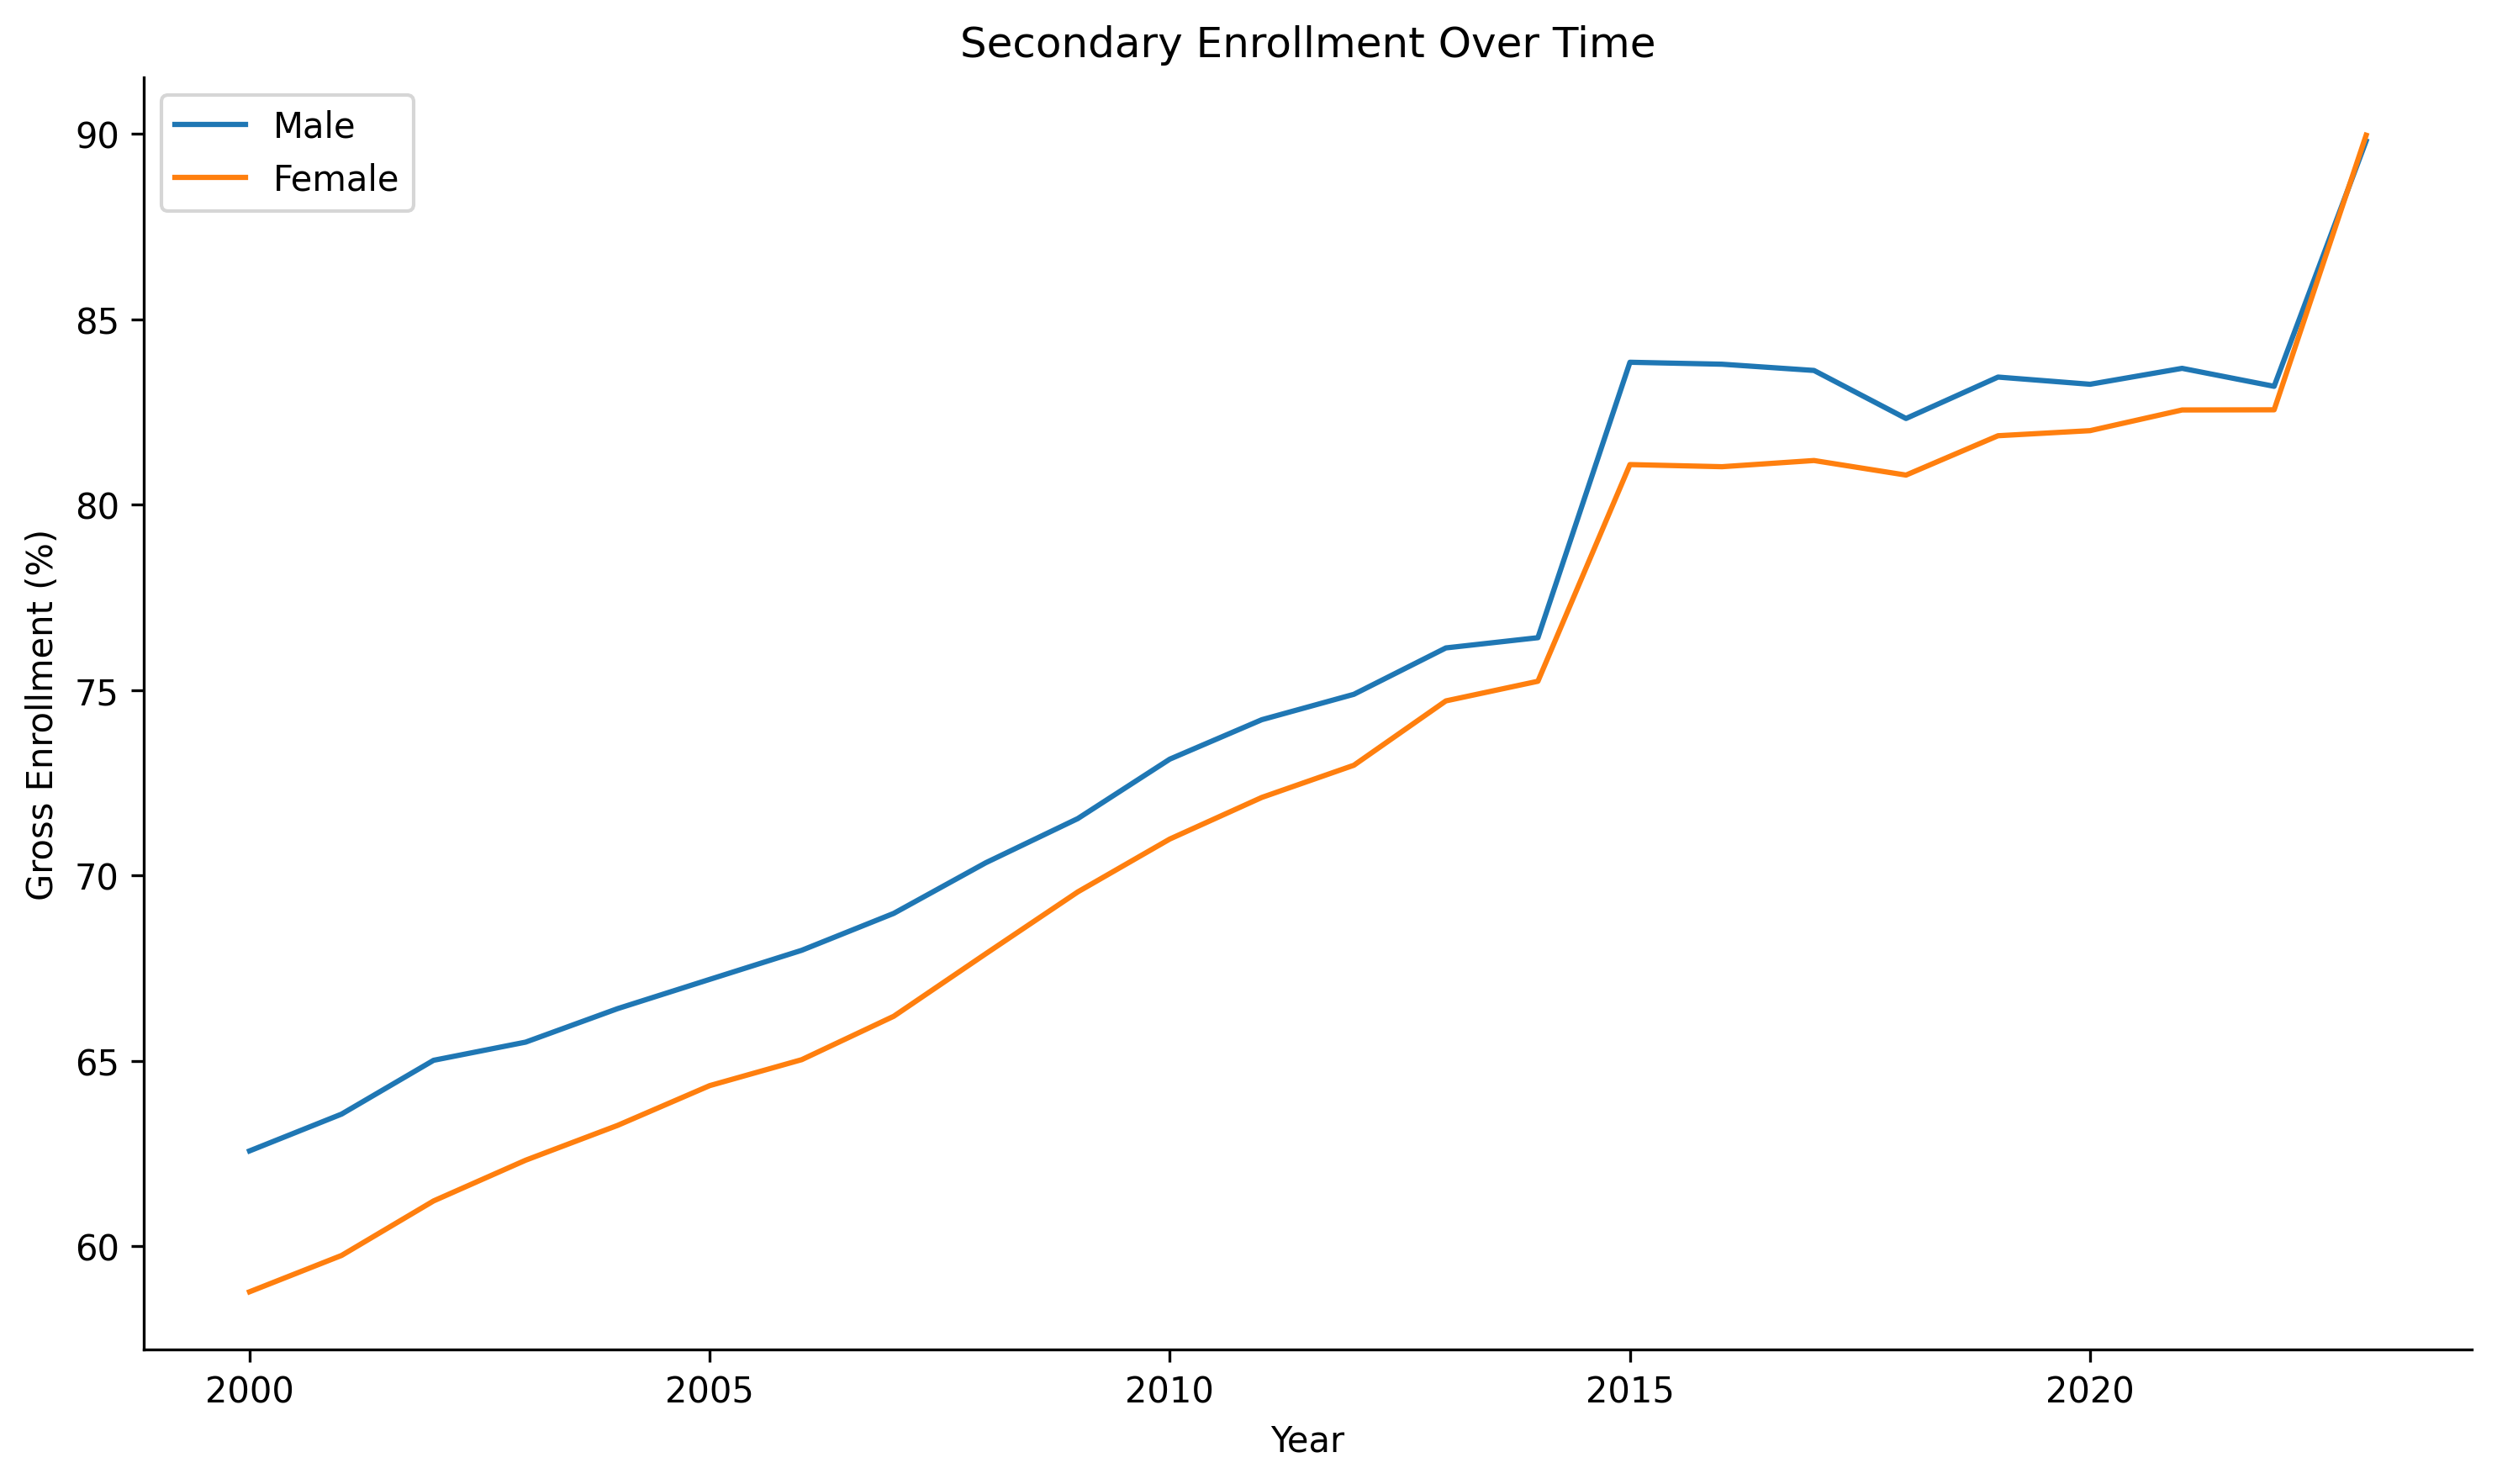
\includegraphics[width=0.95\linewidth,height=\textheight,keepaspectratio]{../figures/secondary_gender_trends.png}

}

\subcaption{Secondary school enrollment trends by gender (2000--2023)}

\end{figure}%

\end{minipage}%
%
\begin{minipage}{0.50\linewidth}

\begin{figure}[H]

{\centering 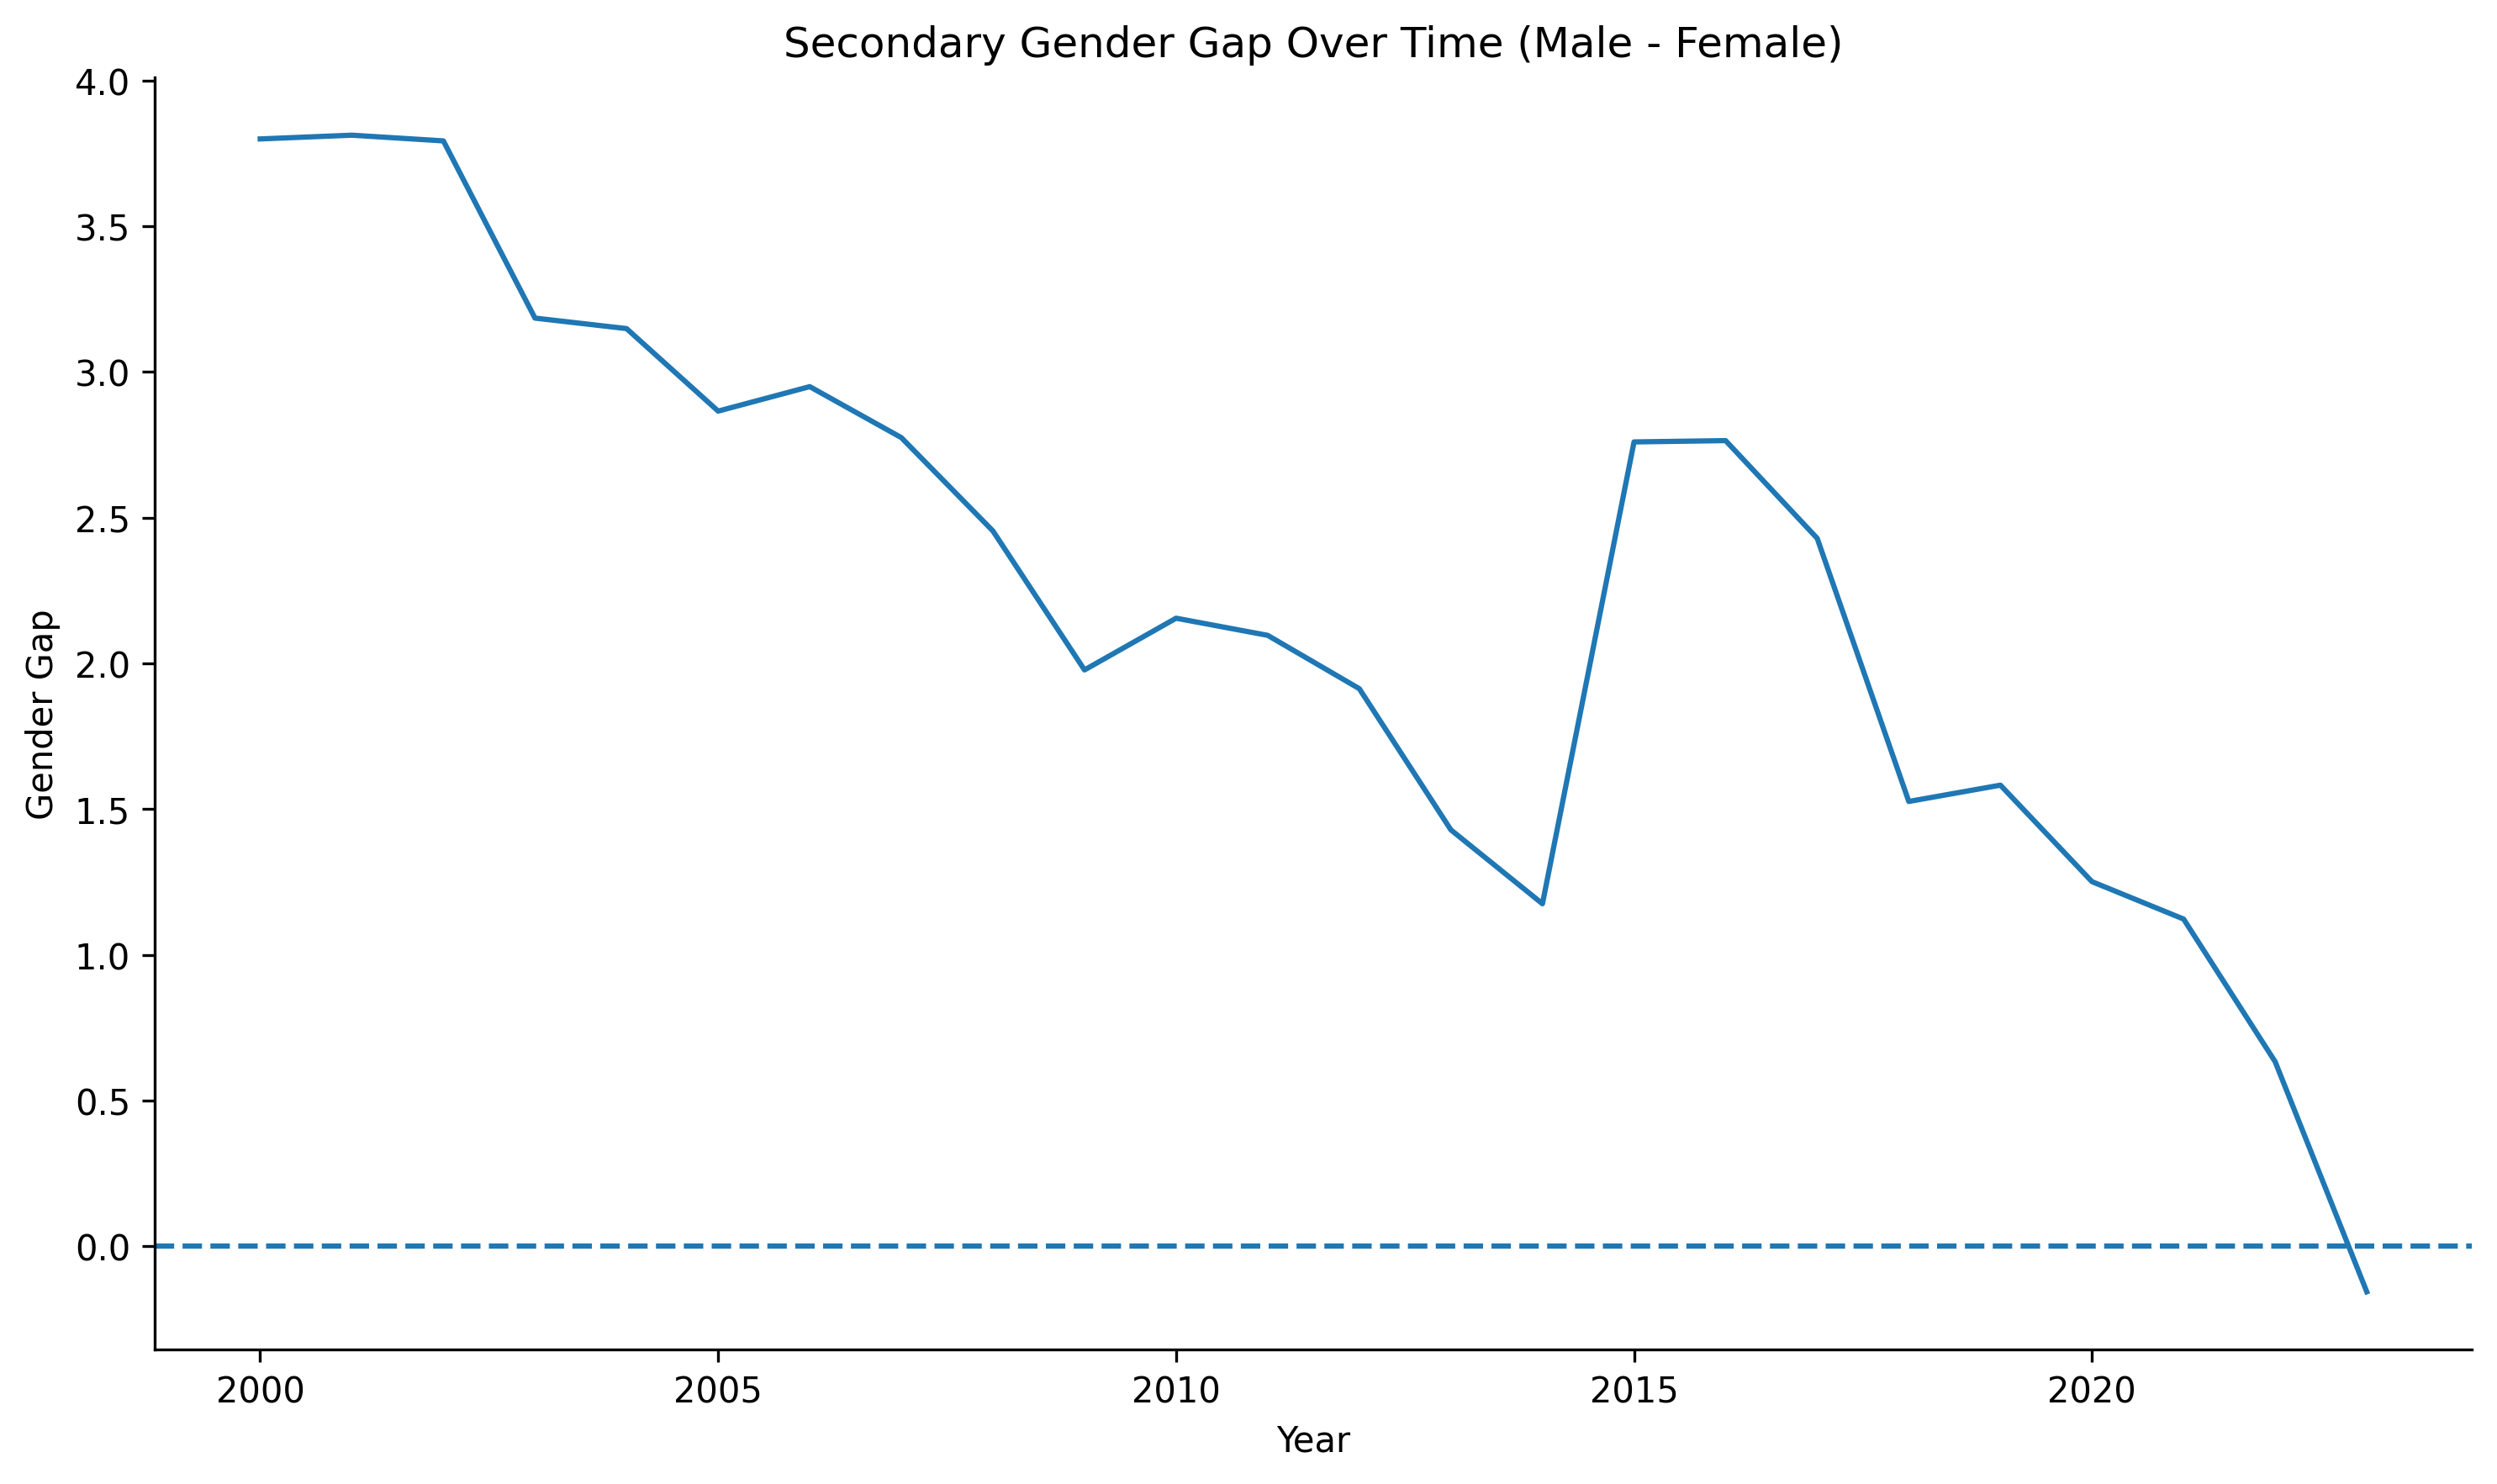
\includegraphics[width=0.95\linewidth,height=\textheight,keepaspectratio]{../figures/secondary_gap_trend.png}

}

\subcaption{Gender gap in secondary enrollment over time}

\end{figure}%

\end{minipage}%

\end{figure}%

\subsubsection{Tertiary Enrollment}\label{tertiary-enrollment}

At the tertiary level, female enrollment has exceeded male enrollment
throughout the entire study period and the gap has been widening
rapidly. In 2000, the gap was already about -2 percentage points
(females ahead), with both genders at around 23--25\%. By 2023, female
enrollment reached approximately 71\% compared to male enrollment of
around 56\%, with the gap widening to nearly -16 percentage points.

\begin{figure}

\begin{minipage}{0.50\linewidth}

\begin{figure}[H]

{\centering 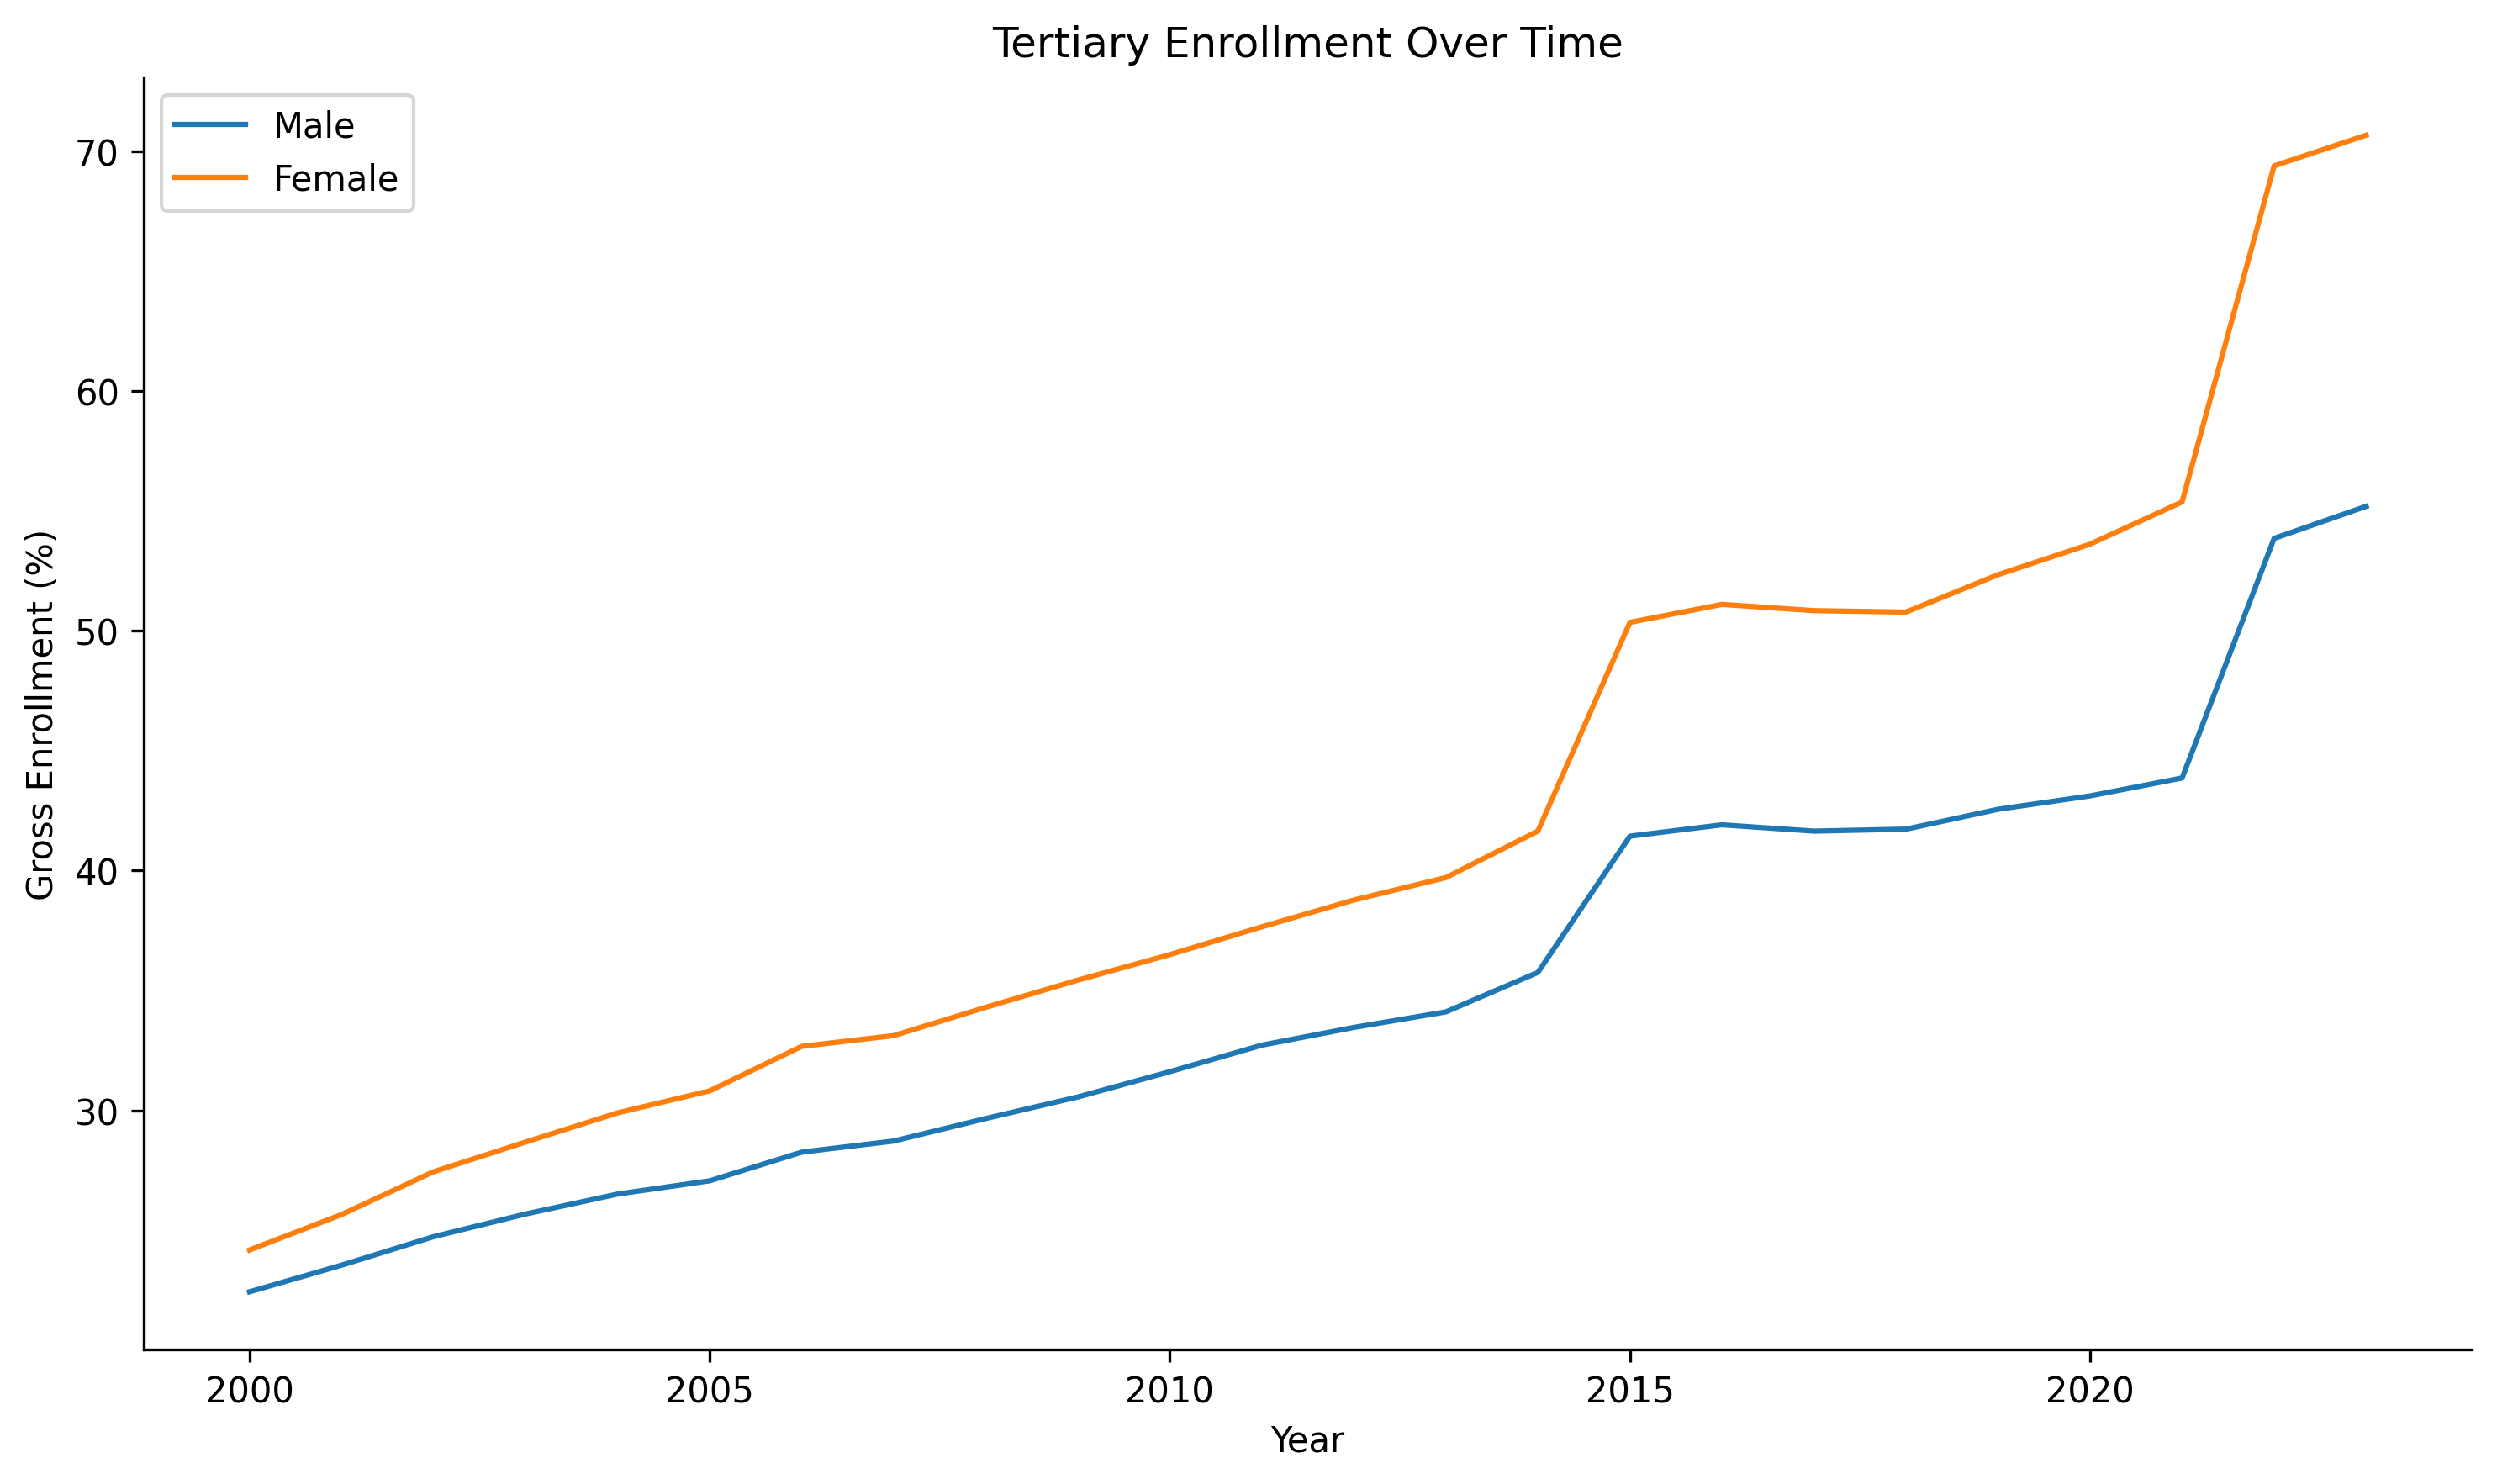
\includegraphics[width=0.95\linewidth,height=\textheight,keepaspectratio]{../figures/tertiary_gender_trends.png}

}

\subcaption{Tertiary school enrollment trends by gender (2000--2023)}

\end{figure}%

\end{minipage}%
%
\begin{minipage}{0.50\linewidth}

\begin{figure}[H]

{\centering 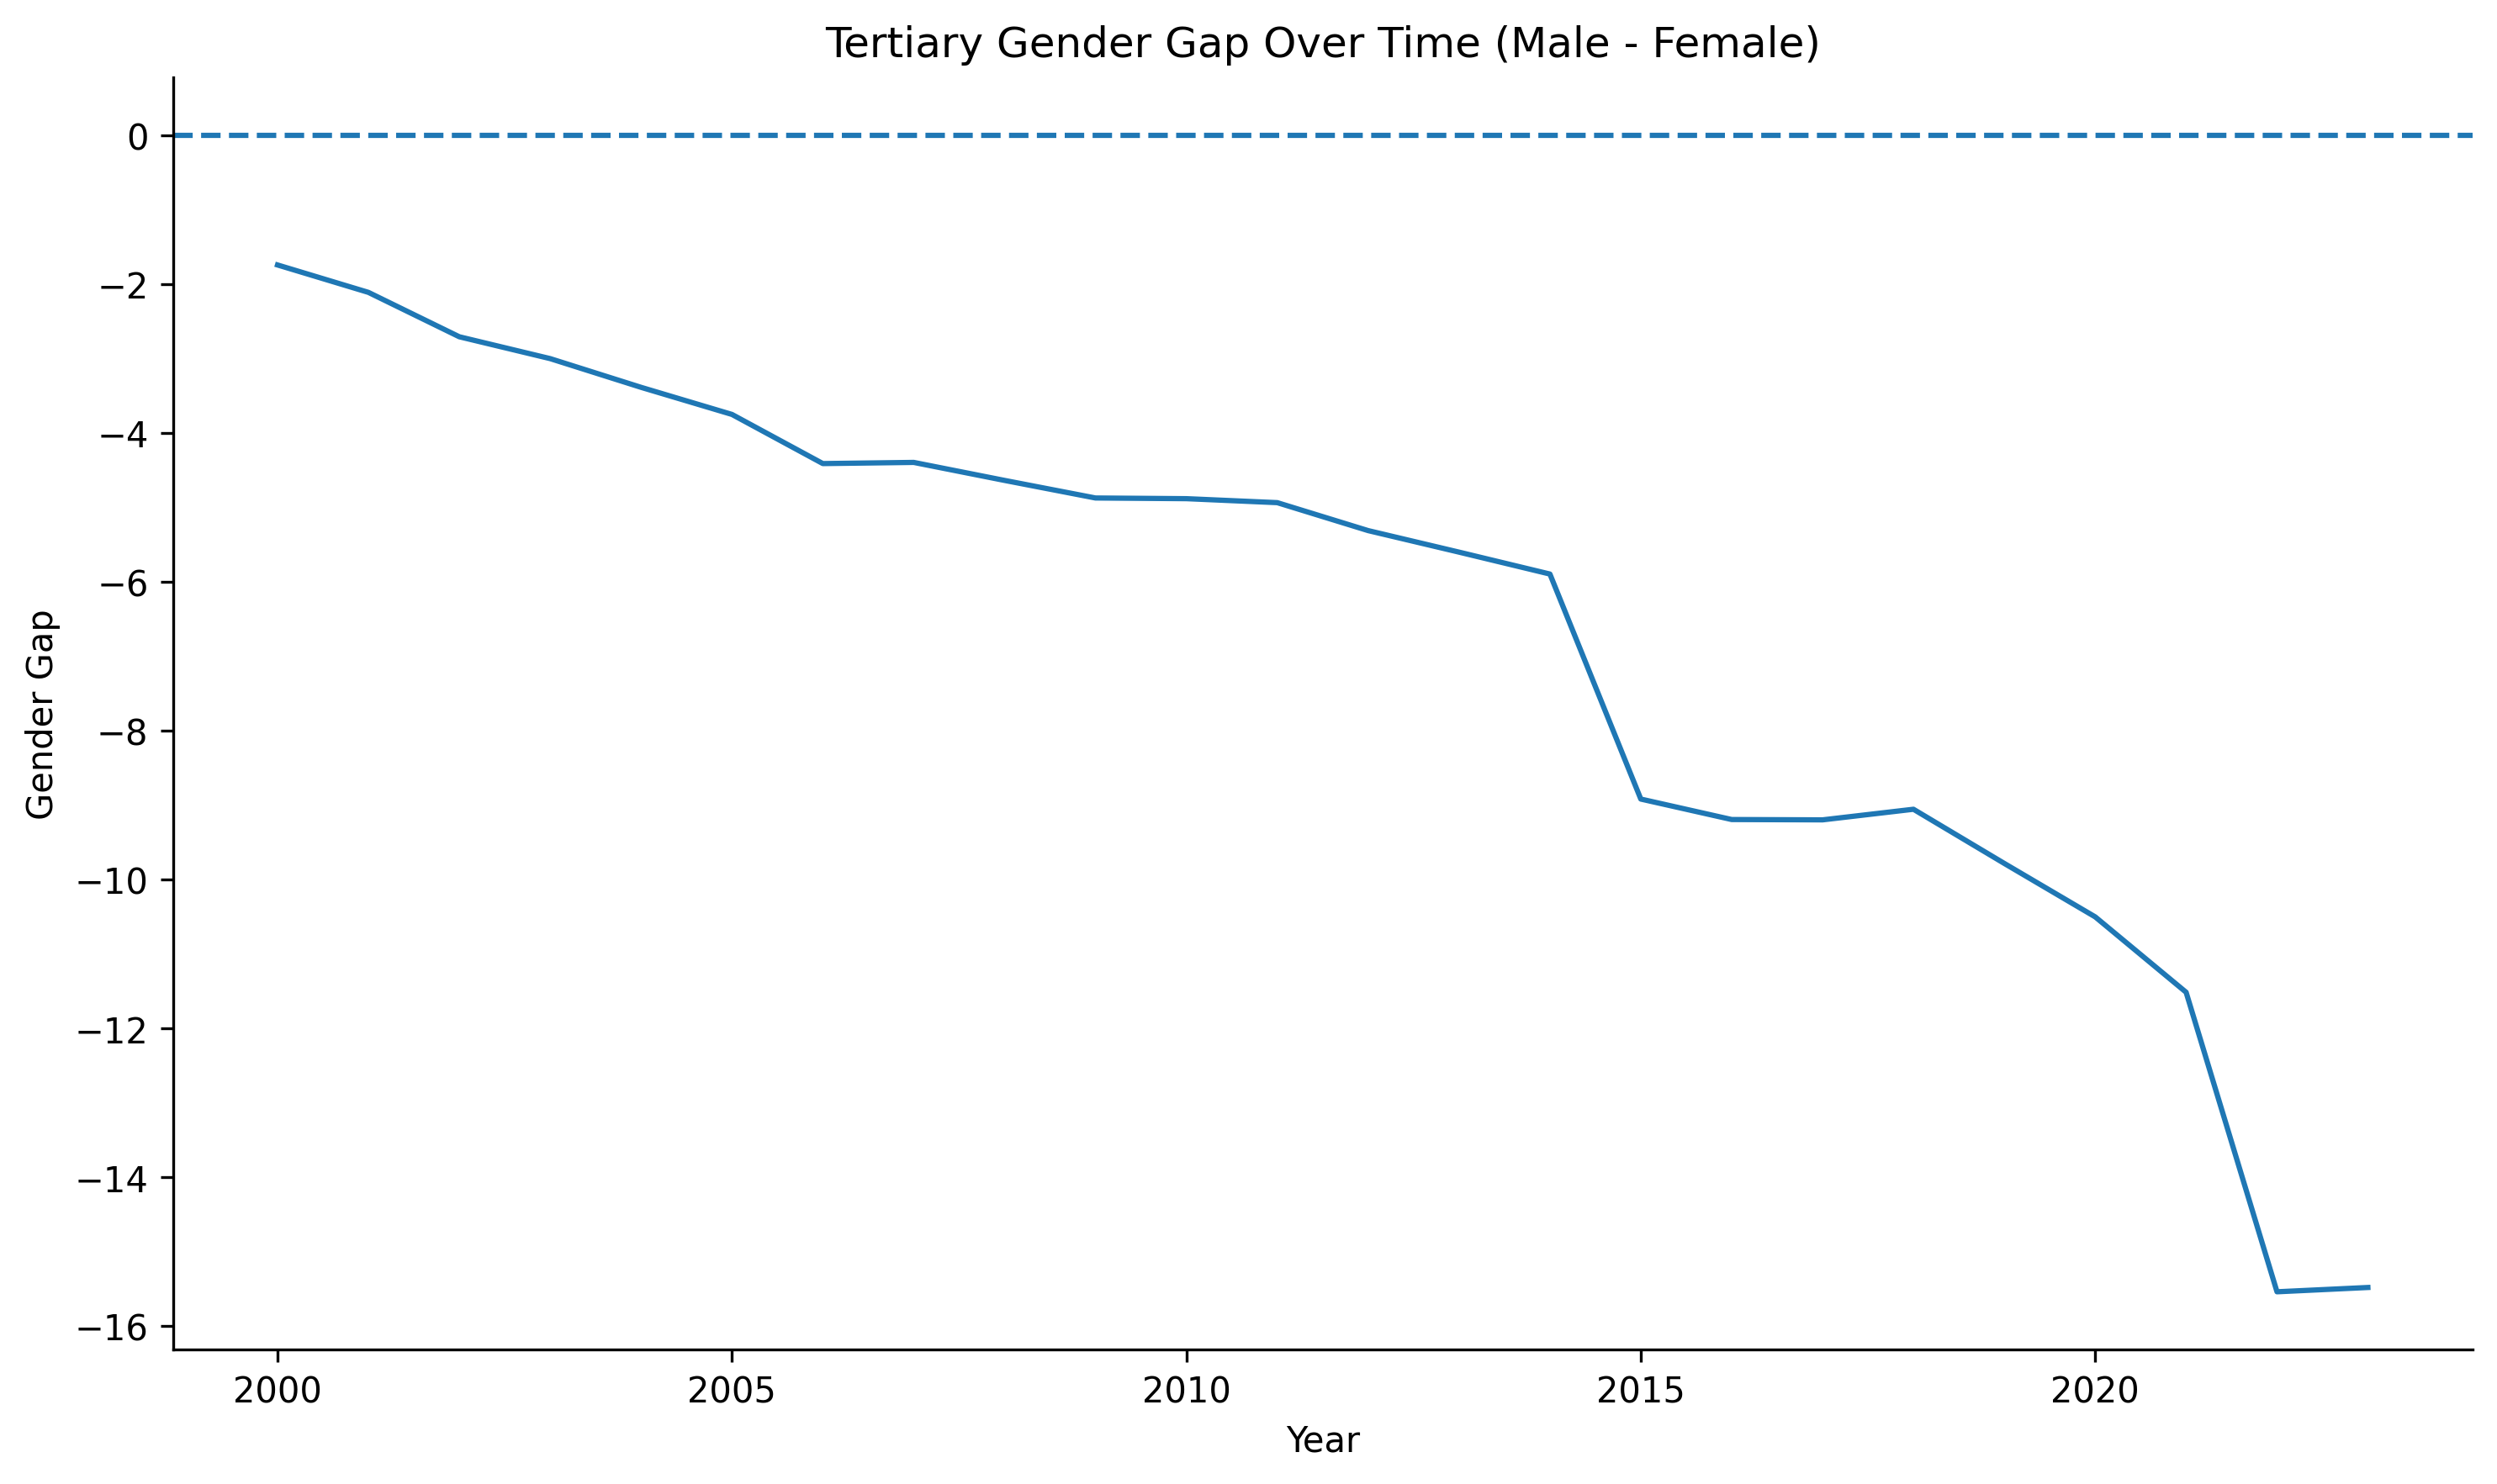
\includegraphics[width=0.95\linewidth,height=\textheight,keepaspectratio]{../figures/tertiary_gap_trend.png}

}

\subcaption{Gender gap in tertiary enrollment over time}

\end{figure}%

\end{minipage}%

\end{figure}%

\subsubsection{Gender Gap Across All Education
Levels}\label{gender-gap-across-all-education-levels}

When comparing all three levels together, primary and secondary gaps
started positive and have converged toward zero, while the tertiary gap
has accelerated downward to about -15 percentage points by 2023. This
suggests that while gender disparities in basic education are narrowing,
a new and growing gap has emerged at the tertiary level in favor of
women.

\begin{figure}[H]

{\centering 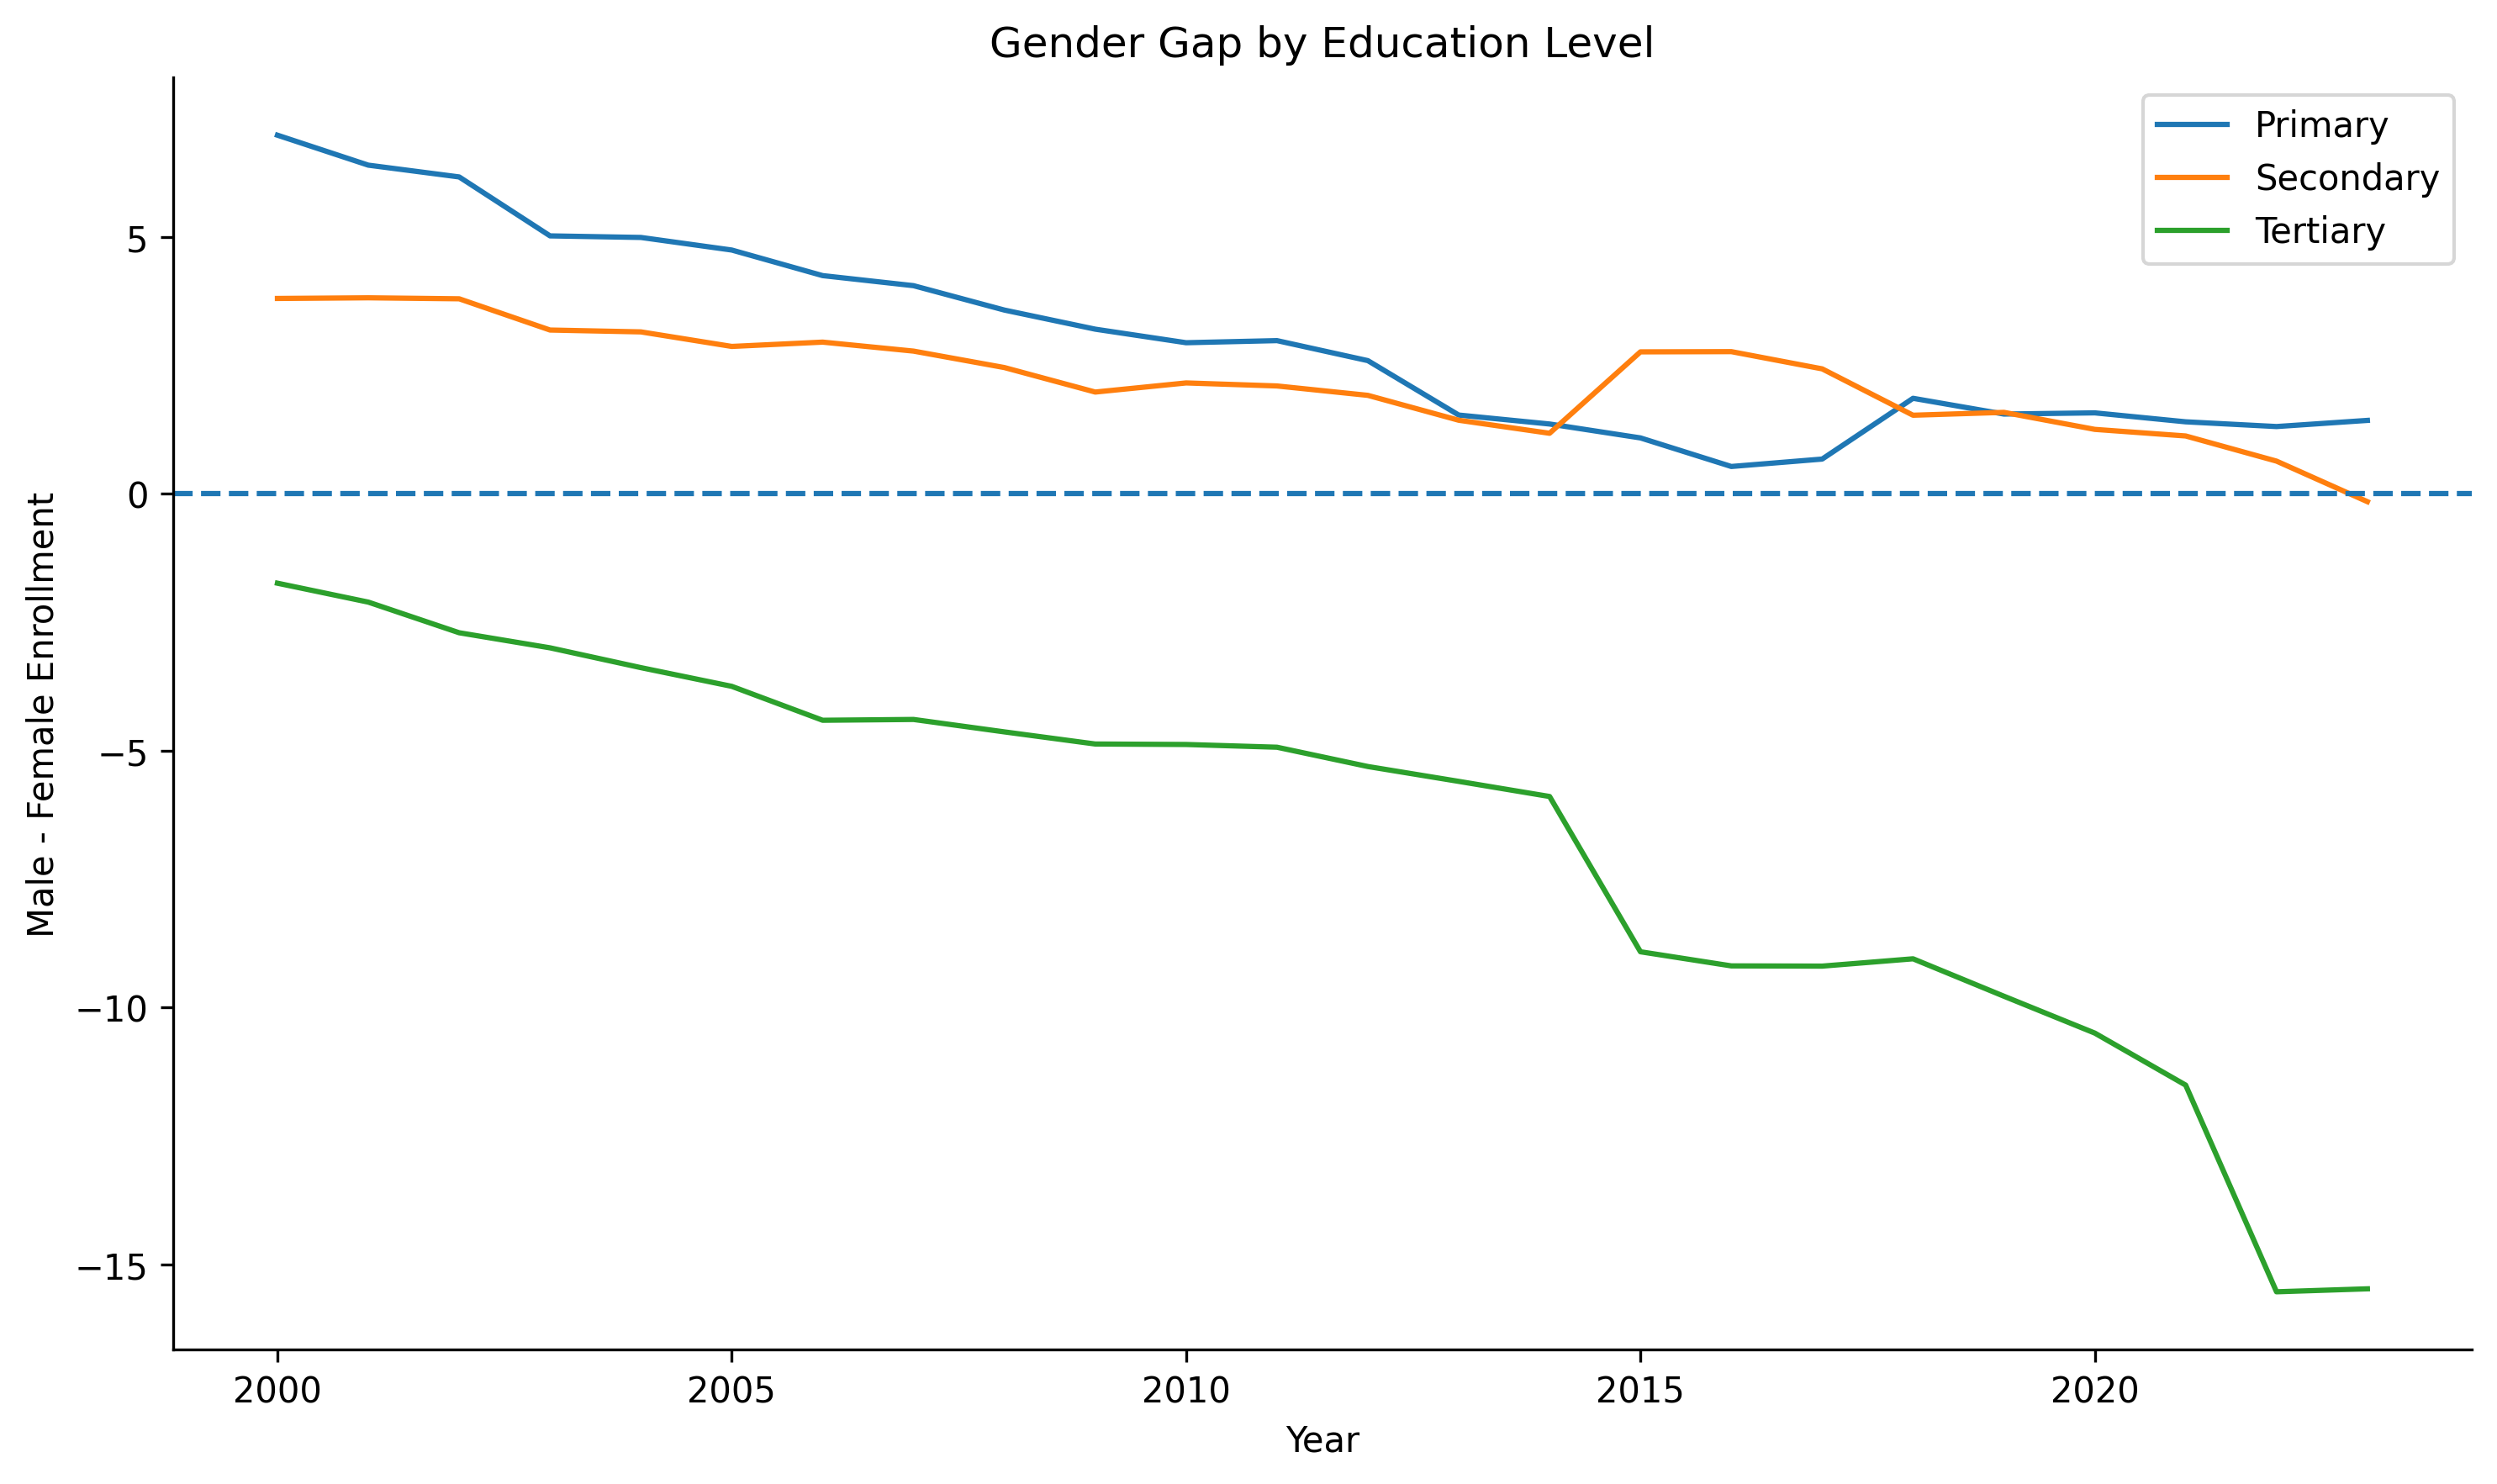
\includegraphics[width=0.65\linewidth,height=\textheight,keepaspectratio]{../figures/gender_gap_by_level.png}

}

\caption{Gender gap across all education levels}

\end{figure}%

\begin{figure}

\begin{minipage}{0.50\linewidth}

\begin{figure}[H]

{\centering 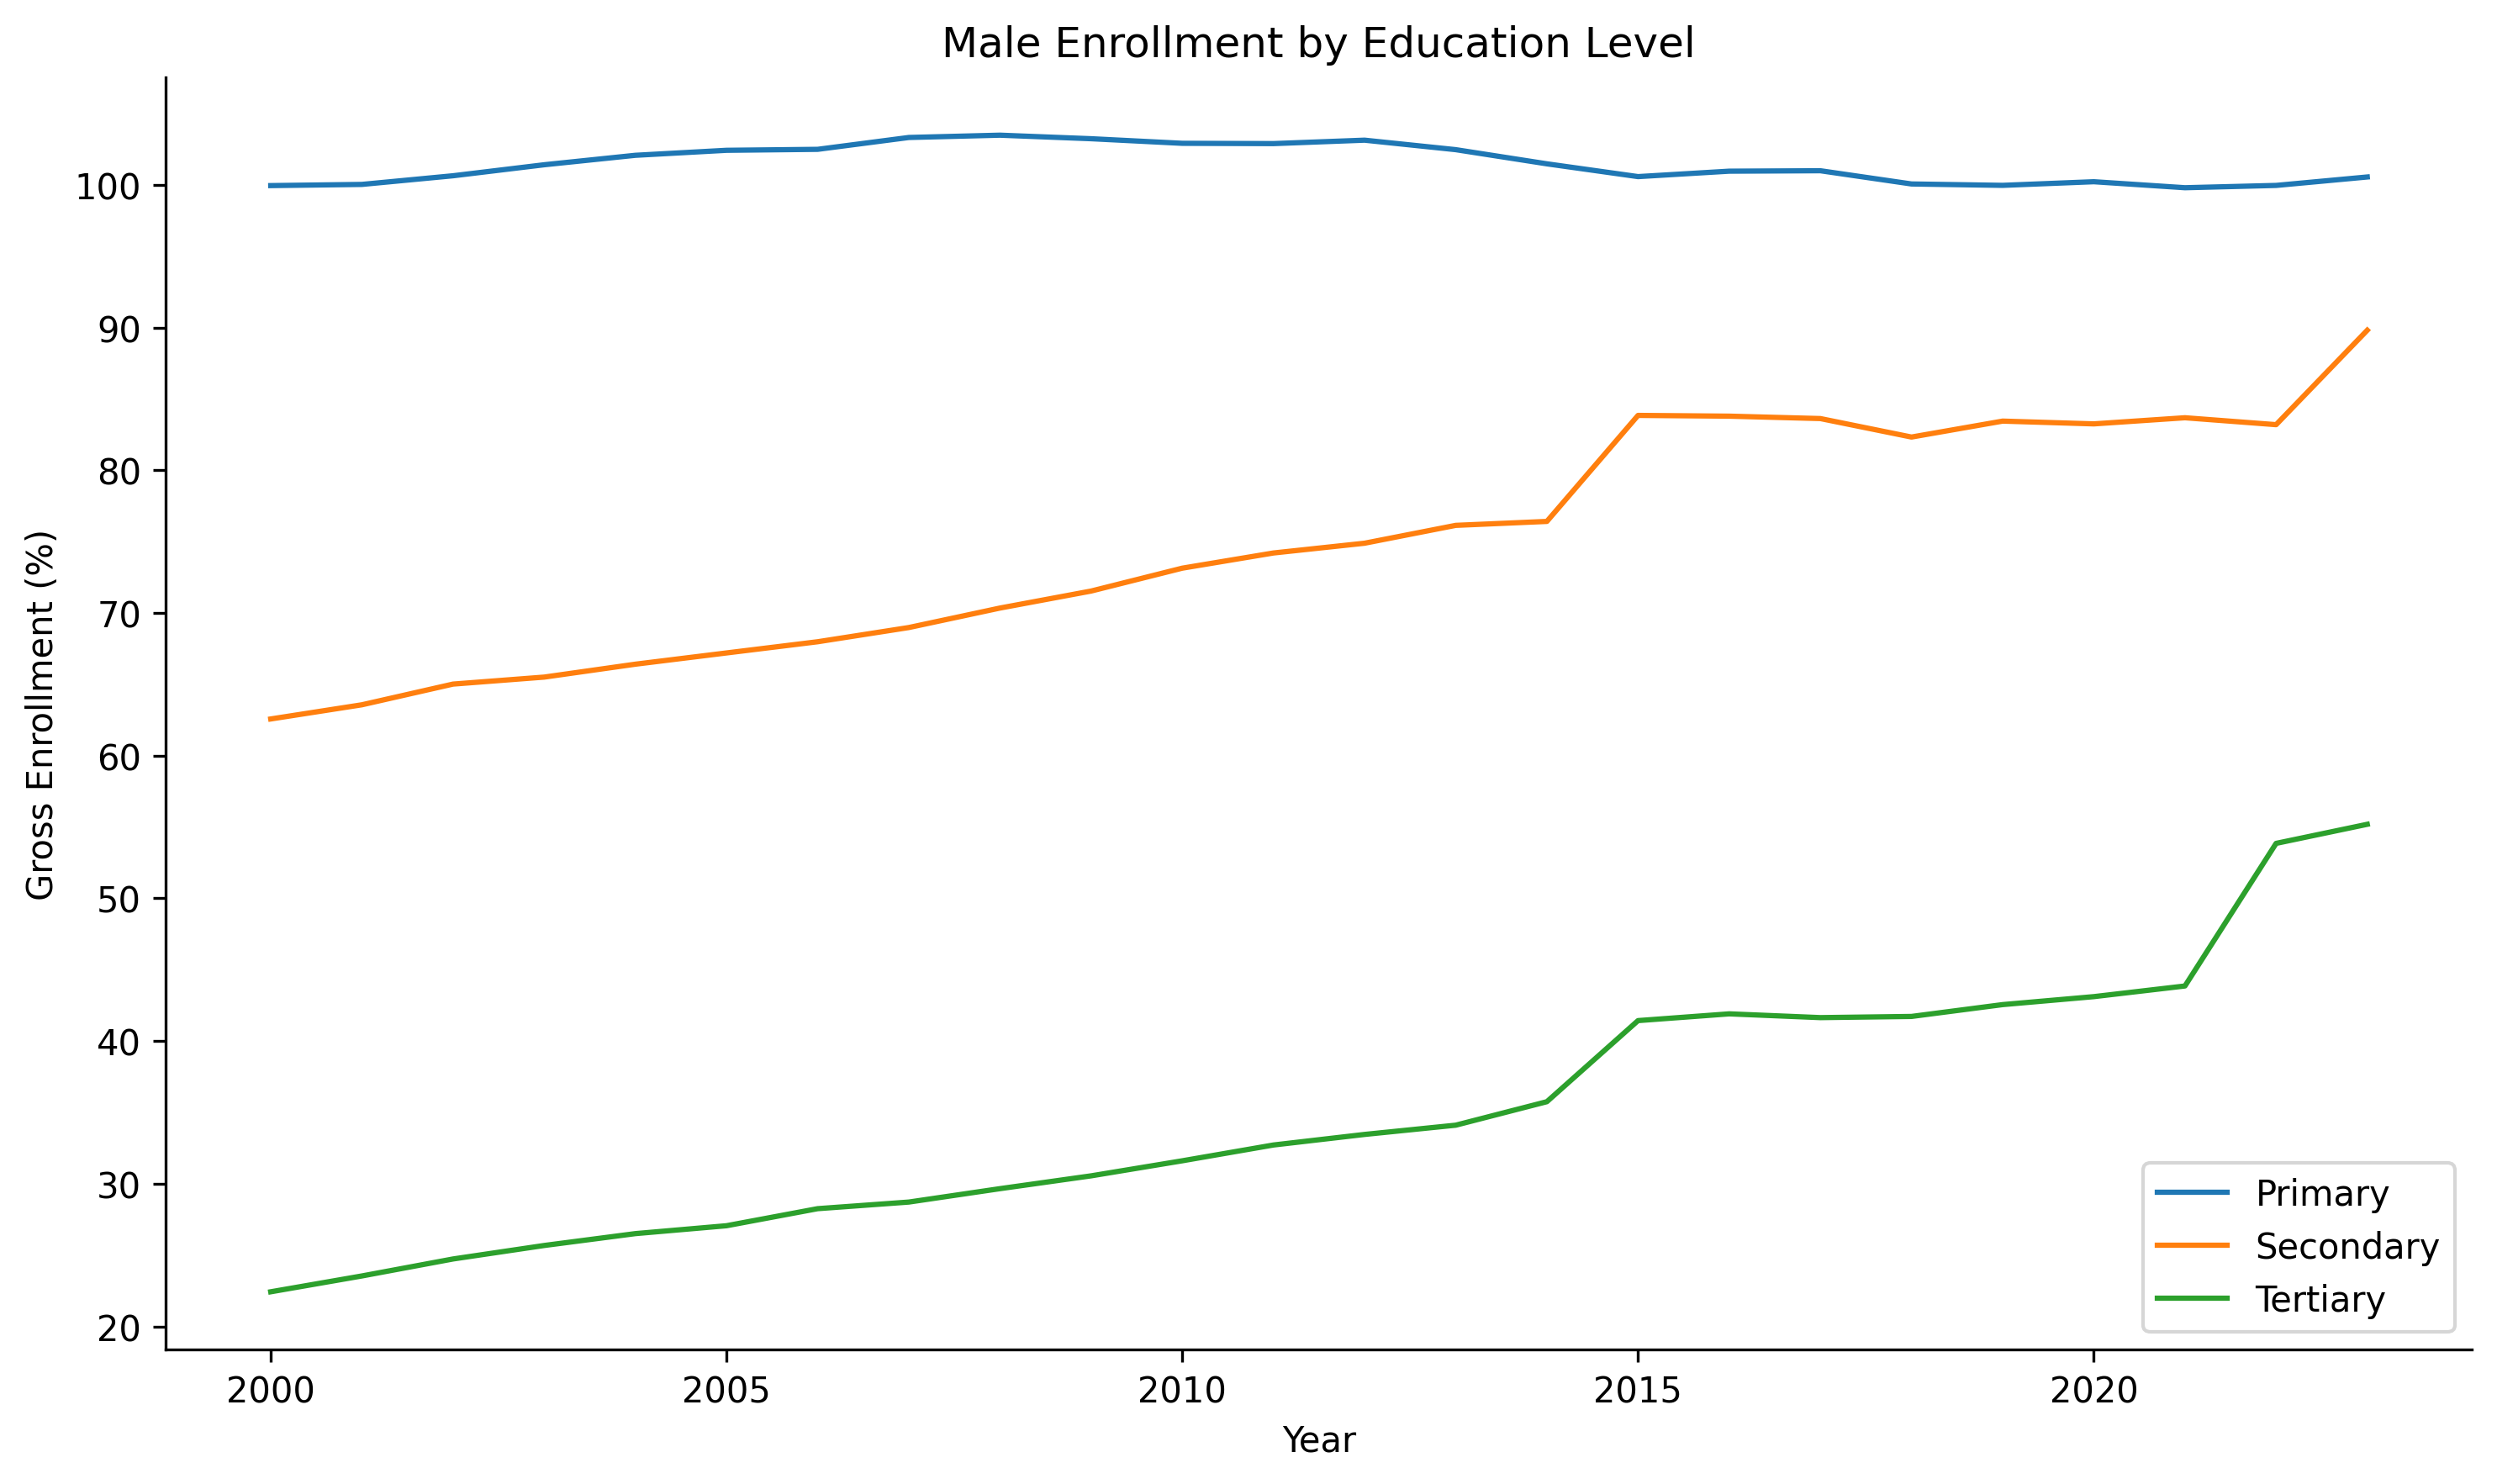
\includegraphics[width=0.95\linewidth,height=\textheight,keepaspectratio]{../figures/male_enrollment_by_level.png}

}

\subcaption{Male enrollment}

\end{figure}%

\end{minipage}%
%
\begin{minipage}{0.50\linewidth}

\begin{figure}[H]

{\centering 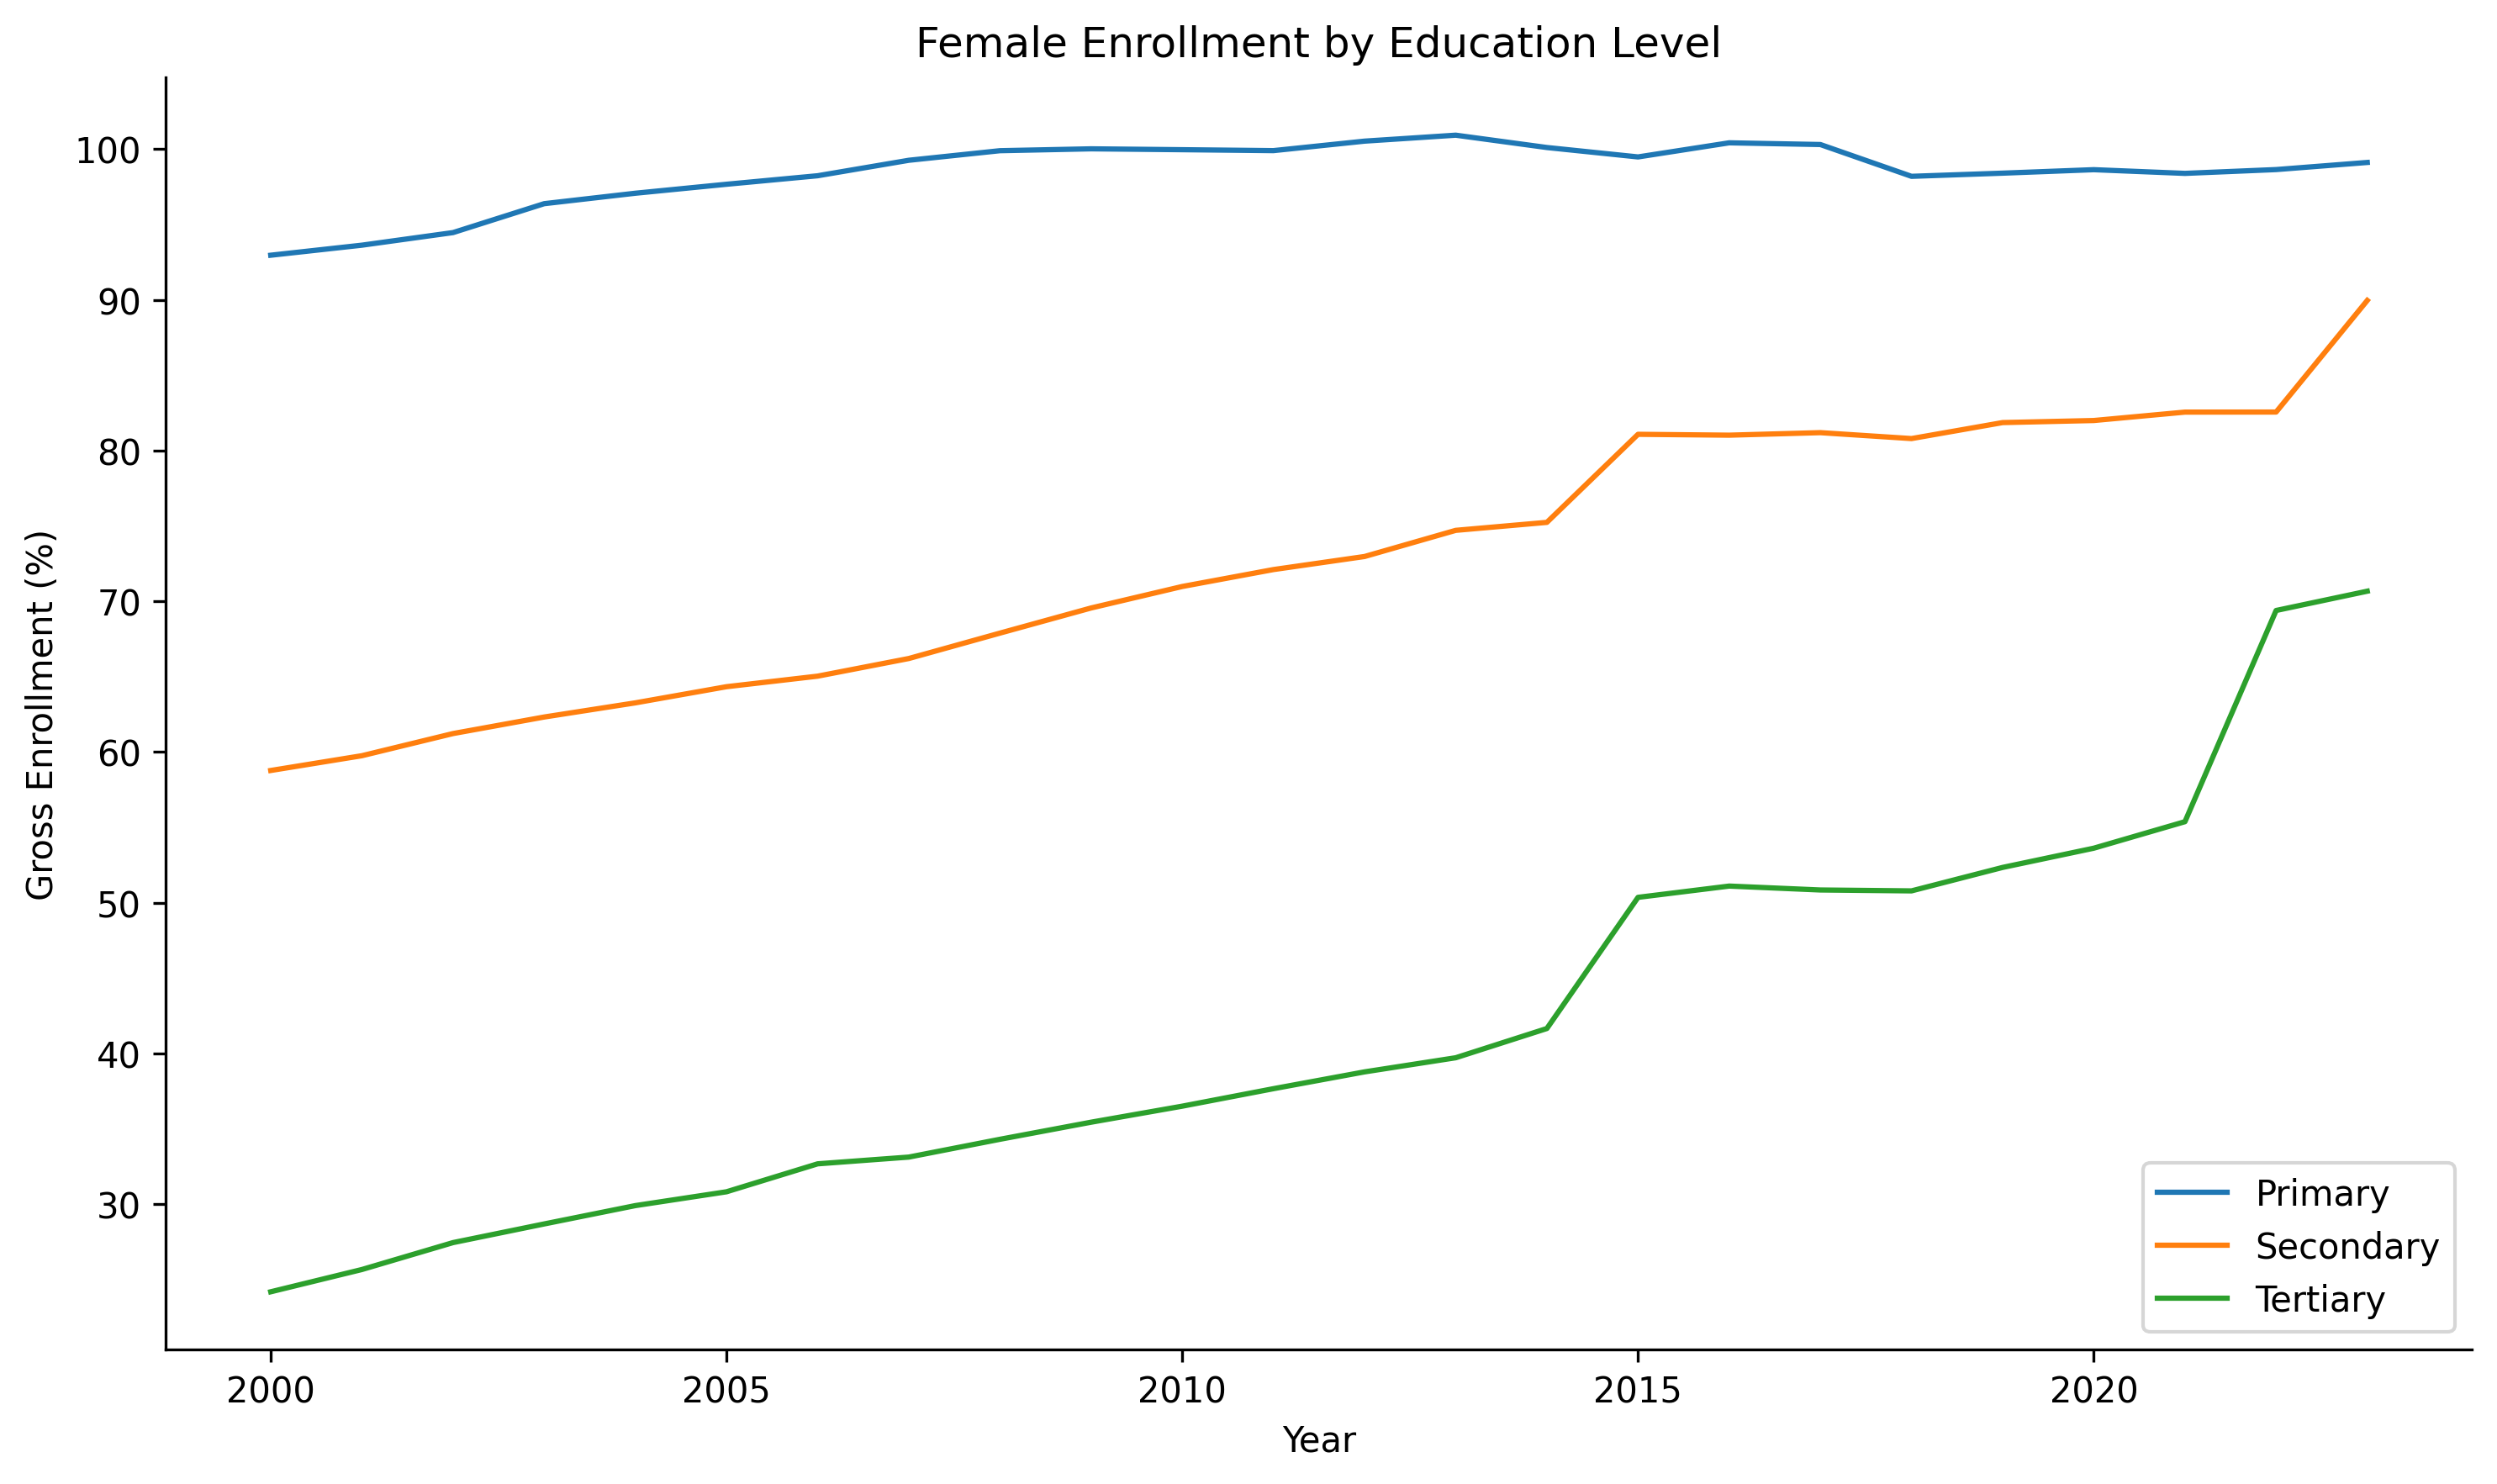
\includegraphics[width=0.95\linewidth,height=\textheight,keepaspectratio]{../figures/female_enrollment_by_level.png}

}

\subcaption{Female enrollment}

\end{figure}%

\end{minipage}%

\end{figure}%

\subsubsection{Regional Breakdown --- Tertiary Enrollment
(2023)}\label{regional-breakdown-tertiary-enrollment-2023}

For female tertiary enrollment in 2023, Australia leads at over 125\%,
followed by North America (\textasciitilde97\%), High income
(\textasciitilde91\%), and the European Union (\textasciitilde89\%).
South Asia (\textasciitilde33\%), Arab World (\textasciitilde35\%), and
Lower middle income (\textasciitilde27\%) have the lowest female
tertiary enrollment. For the tertiary gender gap in 2023, nearly all
regions show negative values. Australia has the largest female advantage
at about -40 percentage points, followed by North America
(\textasciitilde-30) and Latin America \& Caribbean
(\textasciitilde-19). South Asia and Lower middle income are the only
groups near zero.

\begin{figure}

\begin{minipage}{0.50\linewidth}

\begin{figure}[H]

{\centering 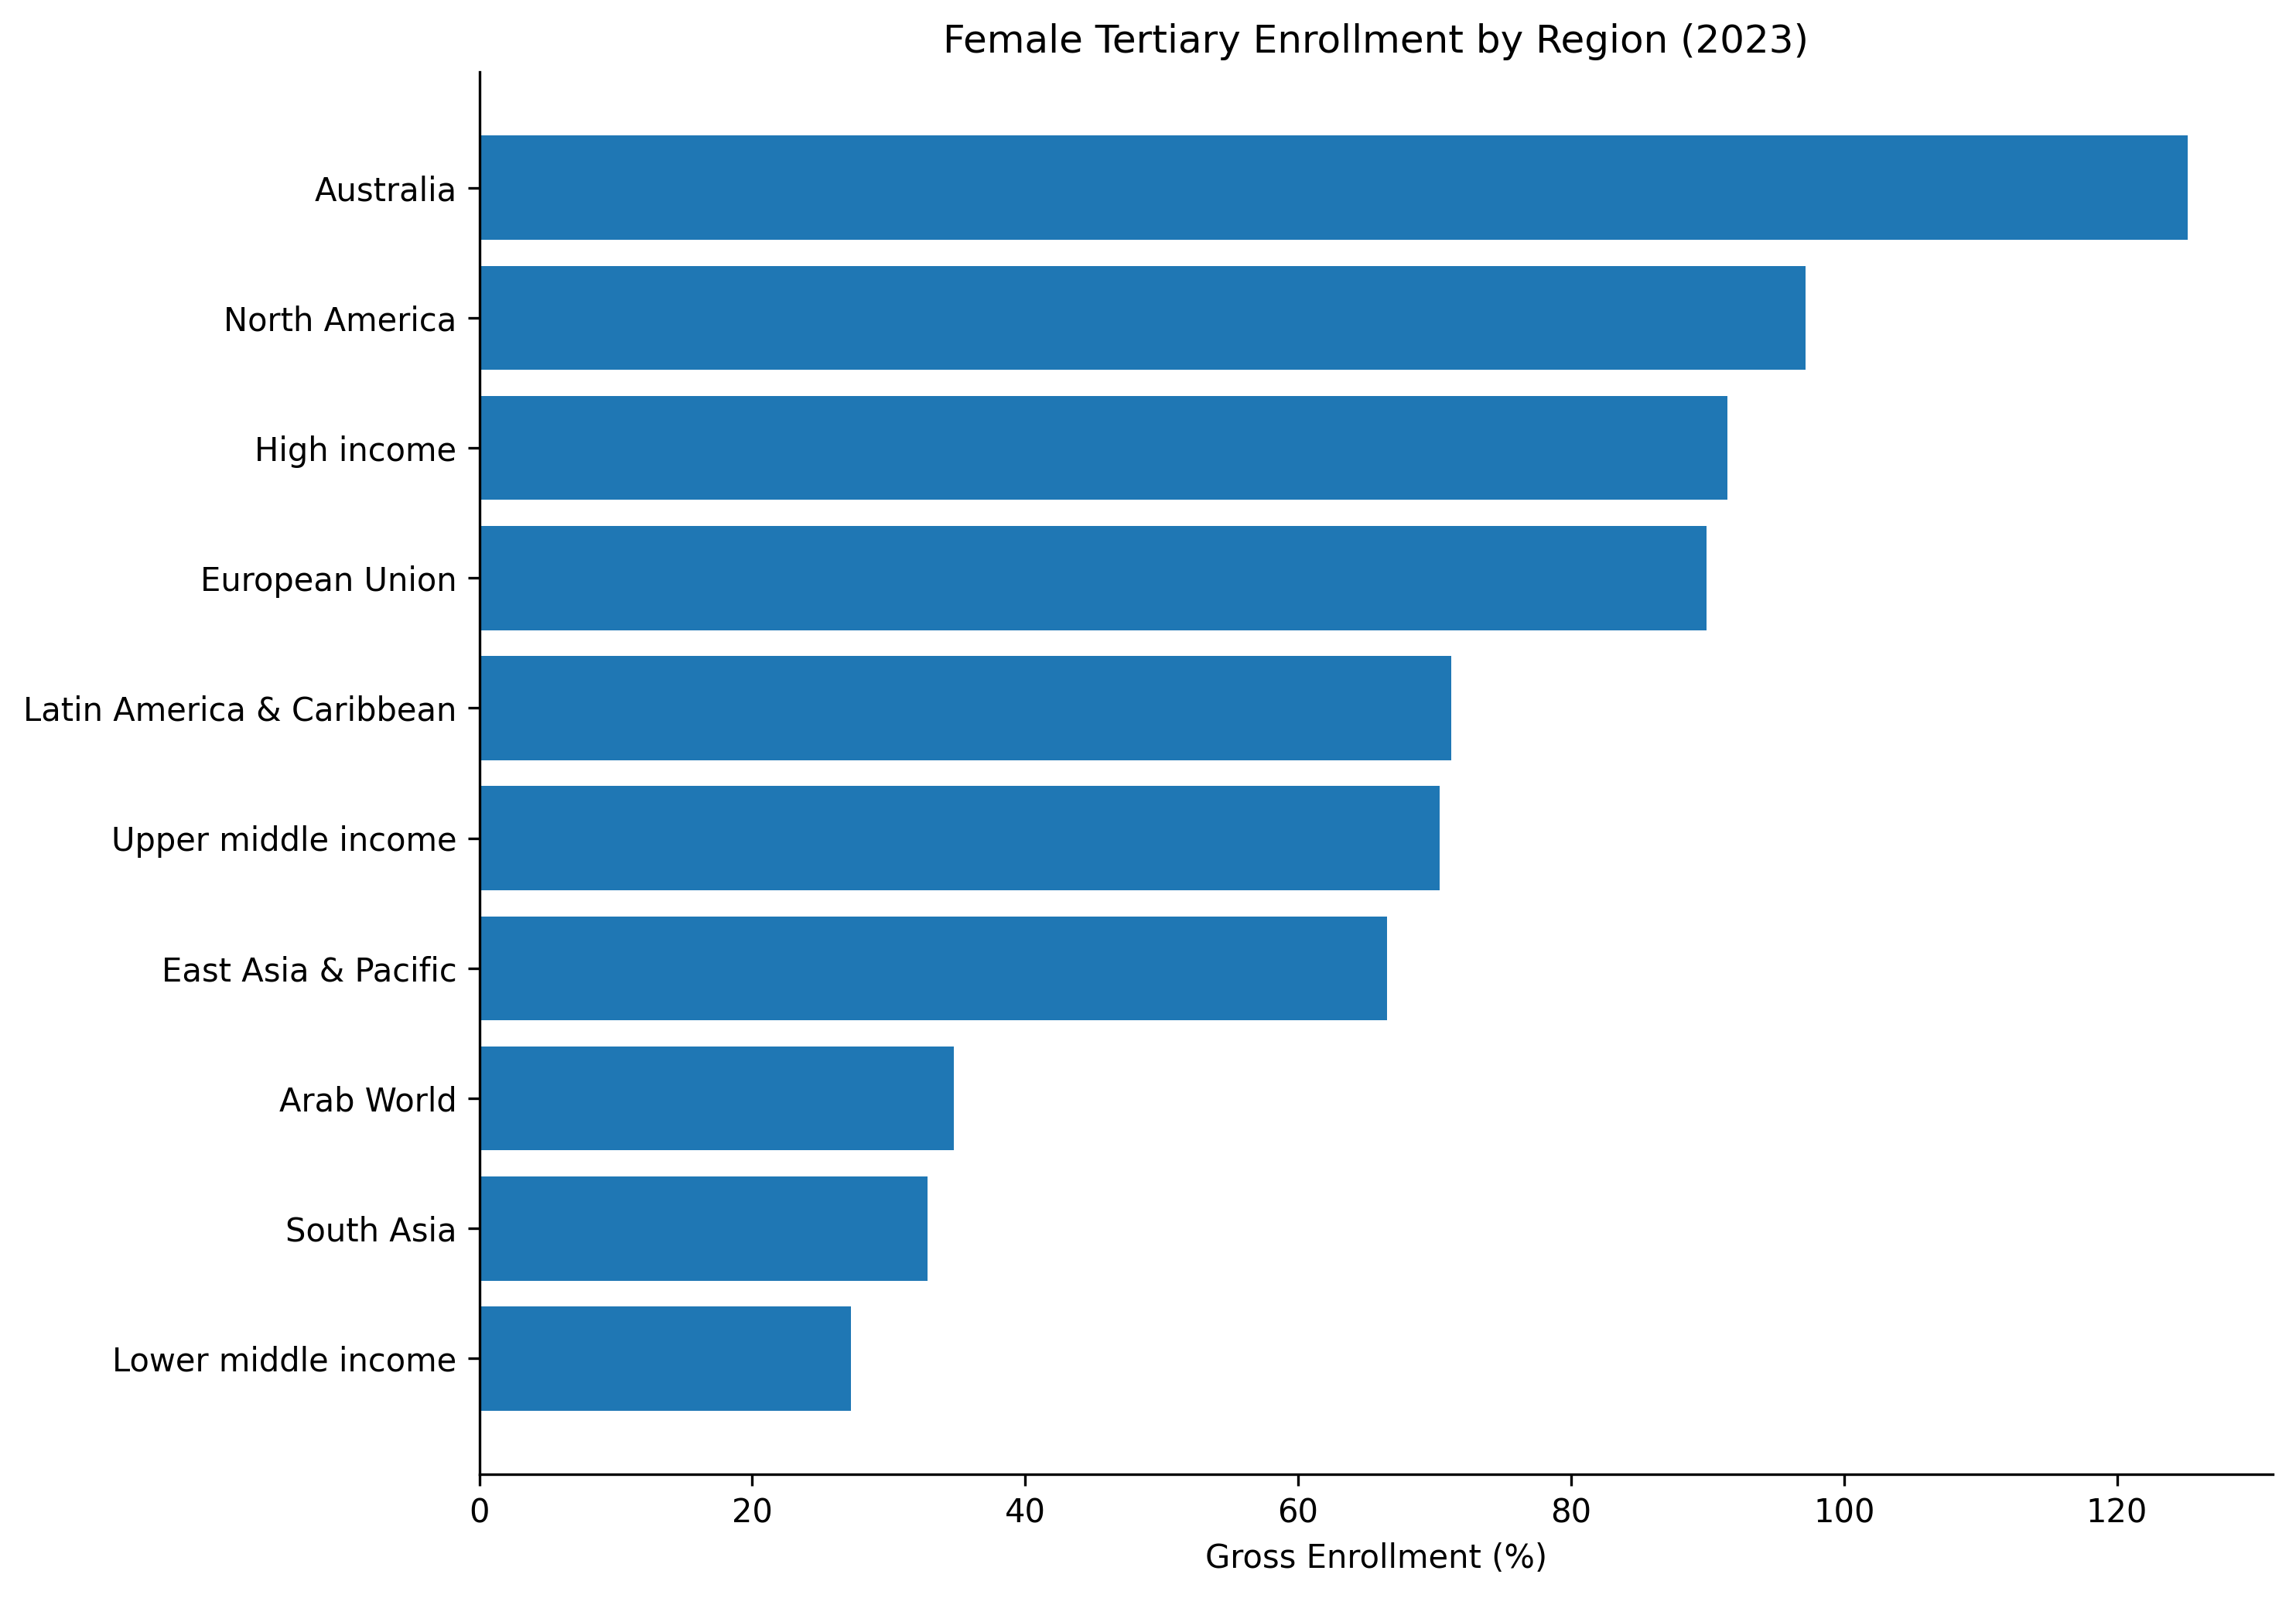
\includegraphics[width=0.95\linewidth,height=\textheight,keepaspectratio]{../figures/female_tertiary_latest_region.png}

}

\subcaption{Female tertiary enrollment by region (2023)}

\end{figure}%

\end{minipage}%
%
\begin{minipage}{0.50\linewidth}

\begin{figure}[H]

{\centering 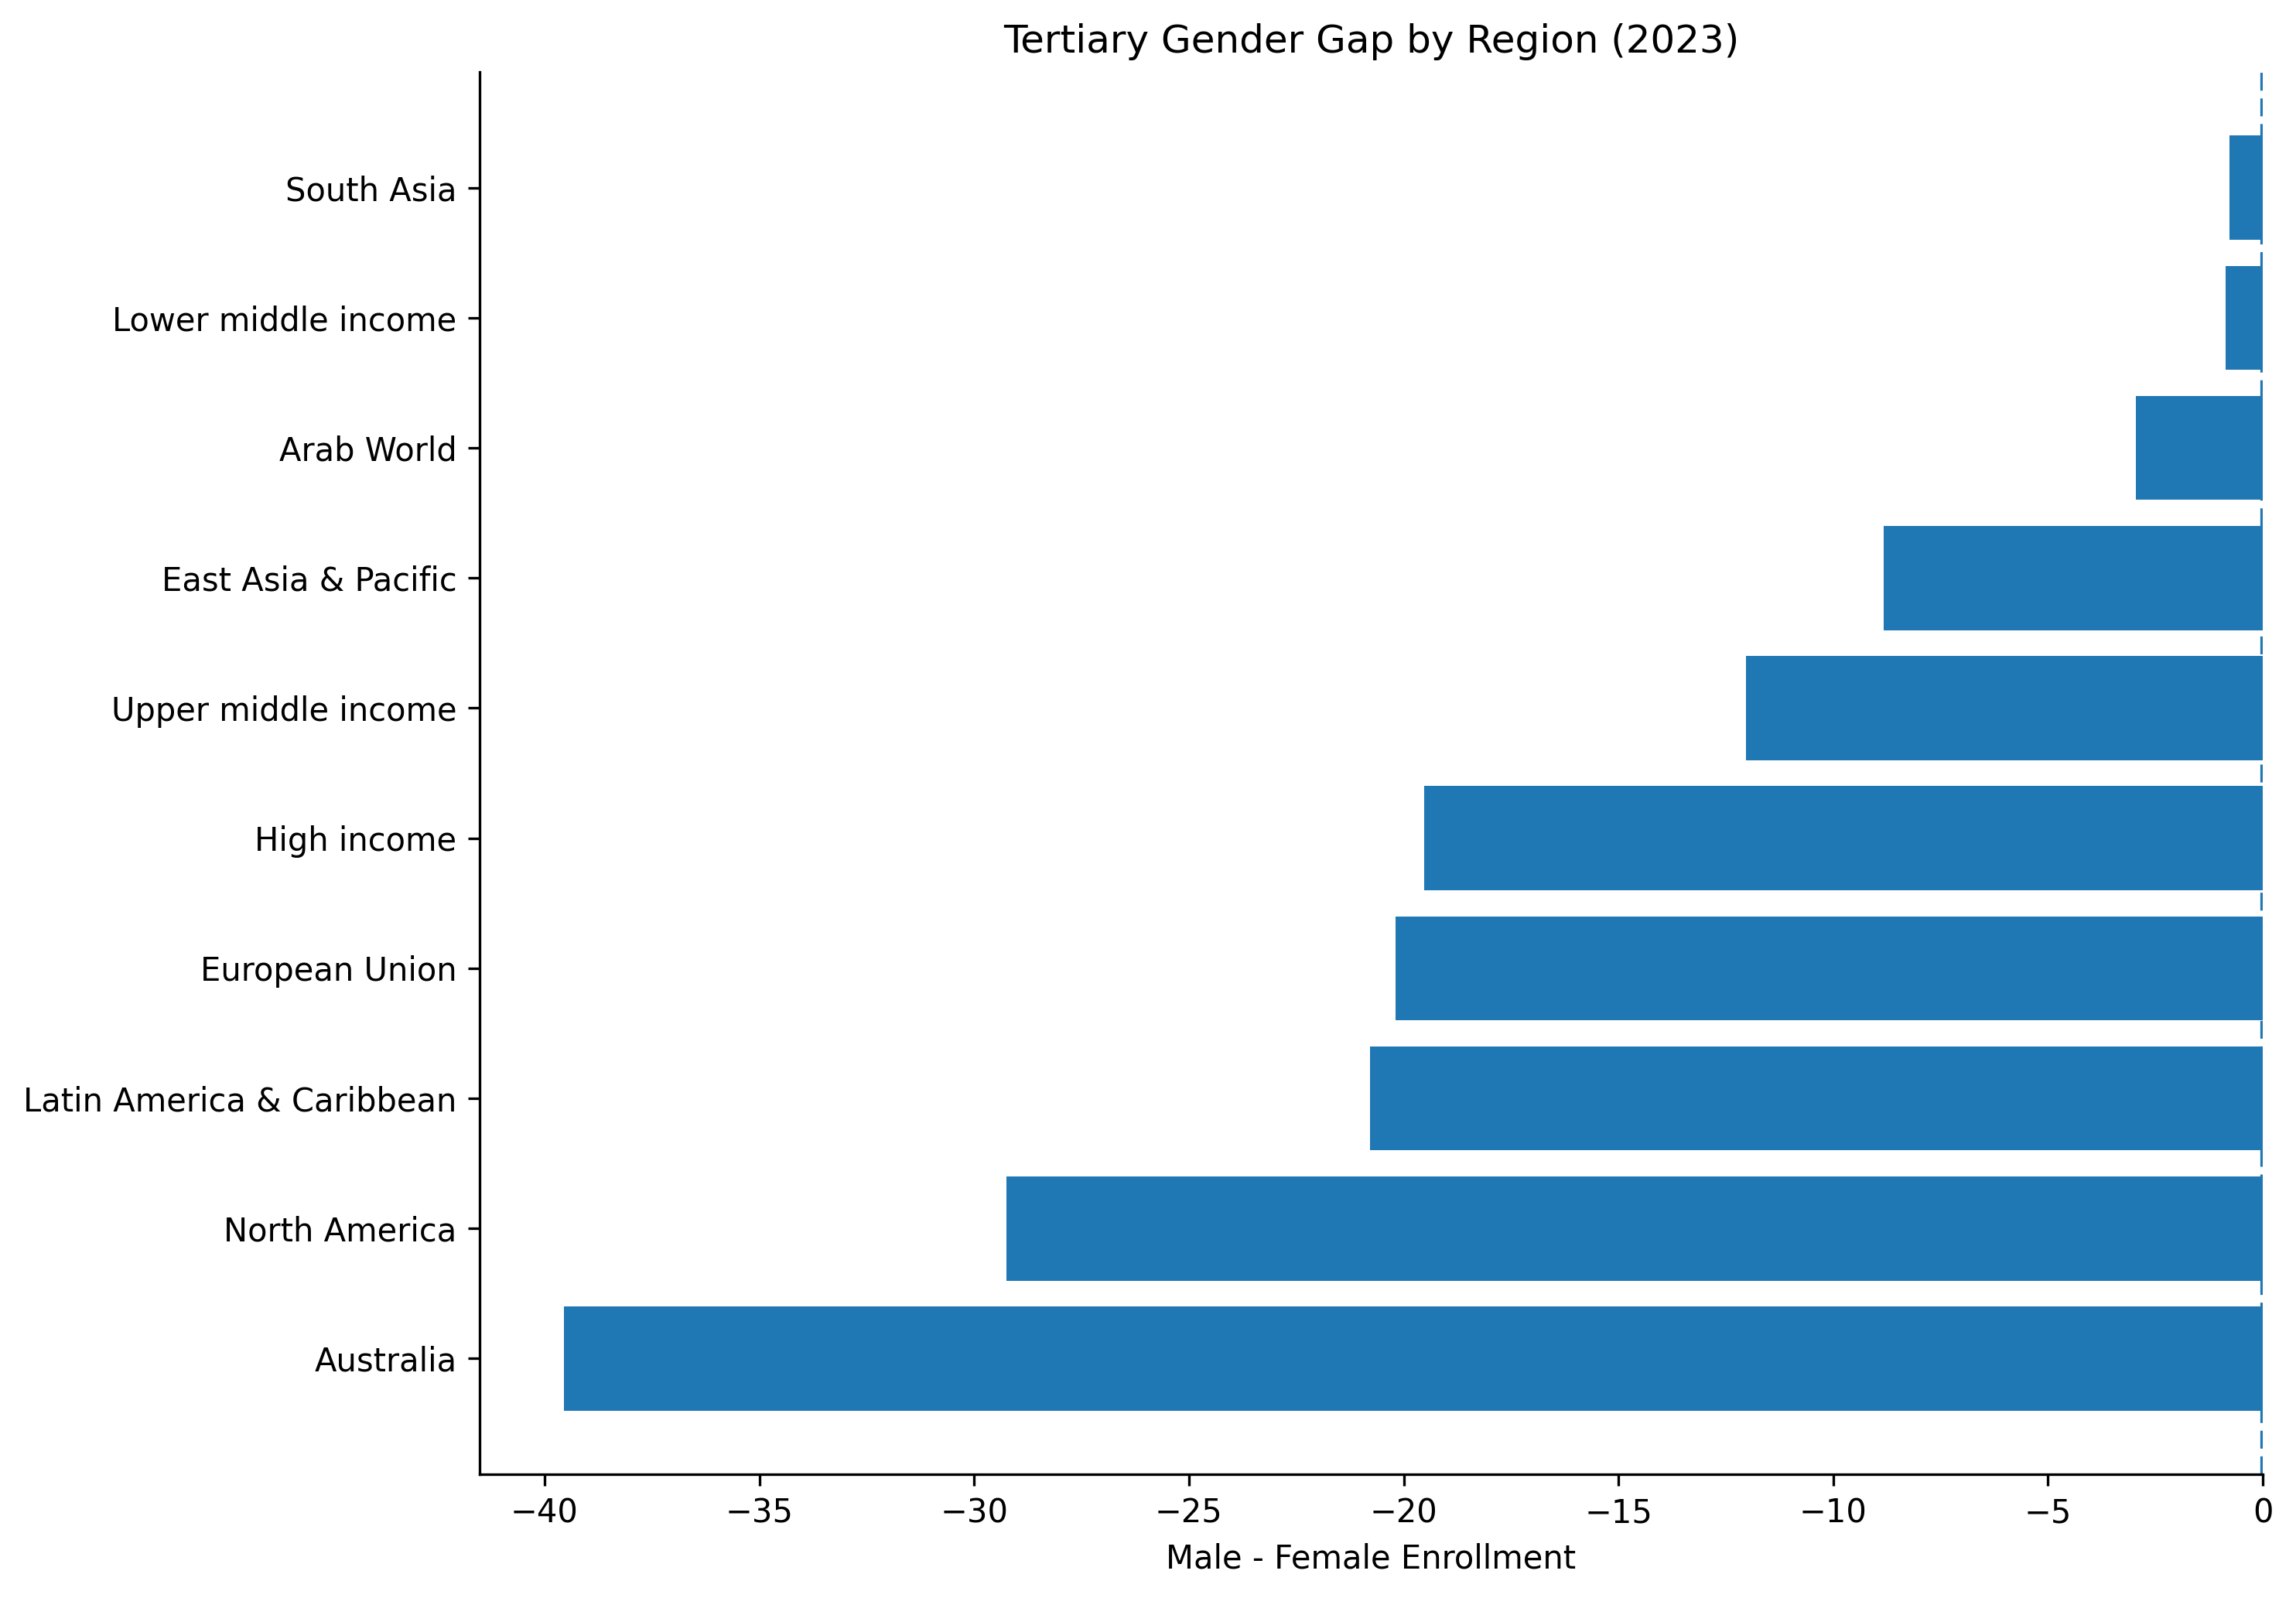
\includegraphics[width=0.95\linewidth,height=\textheight,keepaspectratio]{../figures/tertiary_gap_latest_region.png}

}

\subcaption{Tertiary gender gap by region (2023)}

\end{figure}%

\end{minipage}%

\end{figure}%

\subsubsection{Linear Trend Models}\label{linear-trend-models}

To assess whether enrollment rates have changed systematically over
time, we fit simple linear regression models with year as the predictor
for each gender and education level. These models confirm the visual
trends --- female enrollment shows a positive slope across all three
levels, with the steepest increase at the tertiary level. Male
enrollment trends are flatter at the primary level and positive at
secondary and tertiary, though female slopes are consistently larger,
confirming that female enrollment has been growing faster than male
enrollment across all education levels.

\subsection{RQ2: Trained Teachers and Secondary
Enrollment}\label{rq2-trained-teachers-and-secondary-enrollment}

To address the second research question, we merged the cleaned trained
teacher dataset with the secondary enrollment data on country\_code and
year, then examined the relationship between the percentage of trained
teachers and secondary enrollment rates.

\subsubsection{Relationship Between Trained Teachers and
Enrollment}\label{relationship-between-trained-teachers-and-enrollment}

The scatter plot below shows a clear positive relationship between the
percentage of trained teachers and average secondary enrollment. Regions
with higher proportions of trained teachers tend to have substantially
higher secondary enrollment rates. A linear regression model confirms
this, with a slope of 1.54, an intercept of -51.17, and an R² of 0.709
--- meaning trained teacher percentage explains approximately 71\% of
the variation in average secondary enrollment across regions and years.
The correlation between trained teacher percentage and average
enrollment is 0.849, indicating a strong positive association.
Importantly, this relationship is based on a limited subset of
observations due to missing data and should not be interpreted as
causal.

\begin{figure}[H]

{\centering 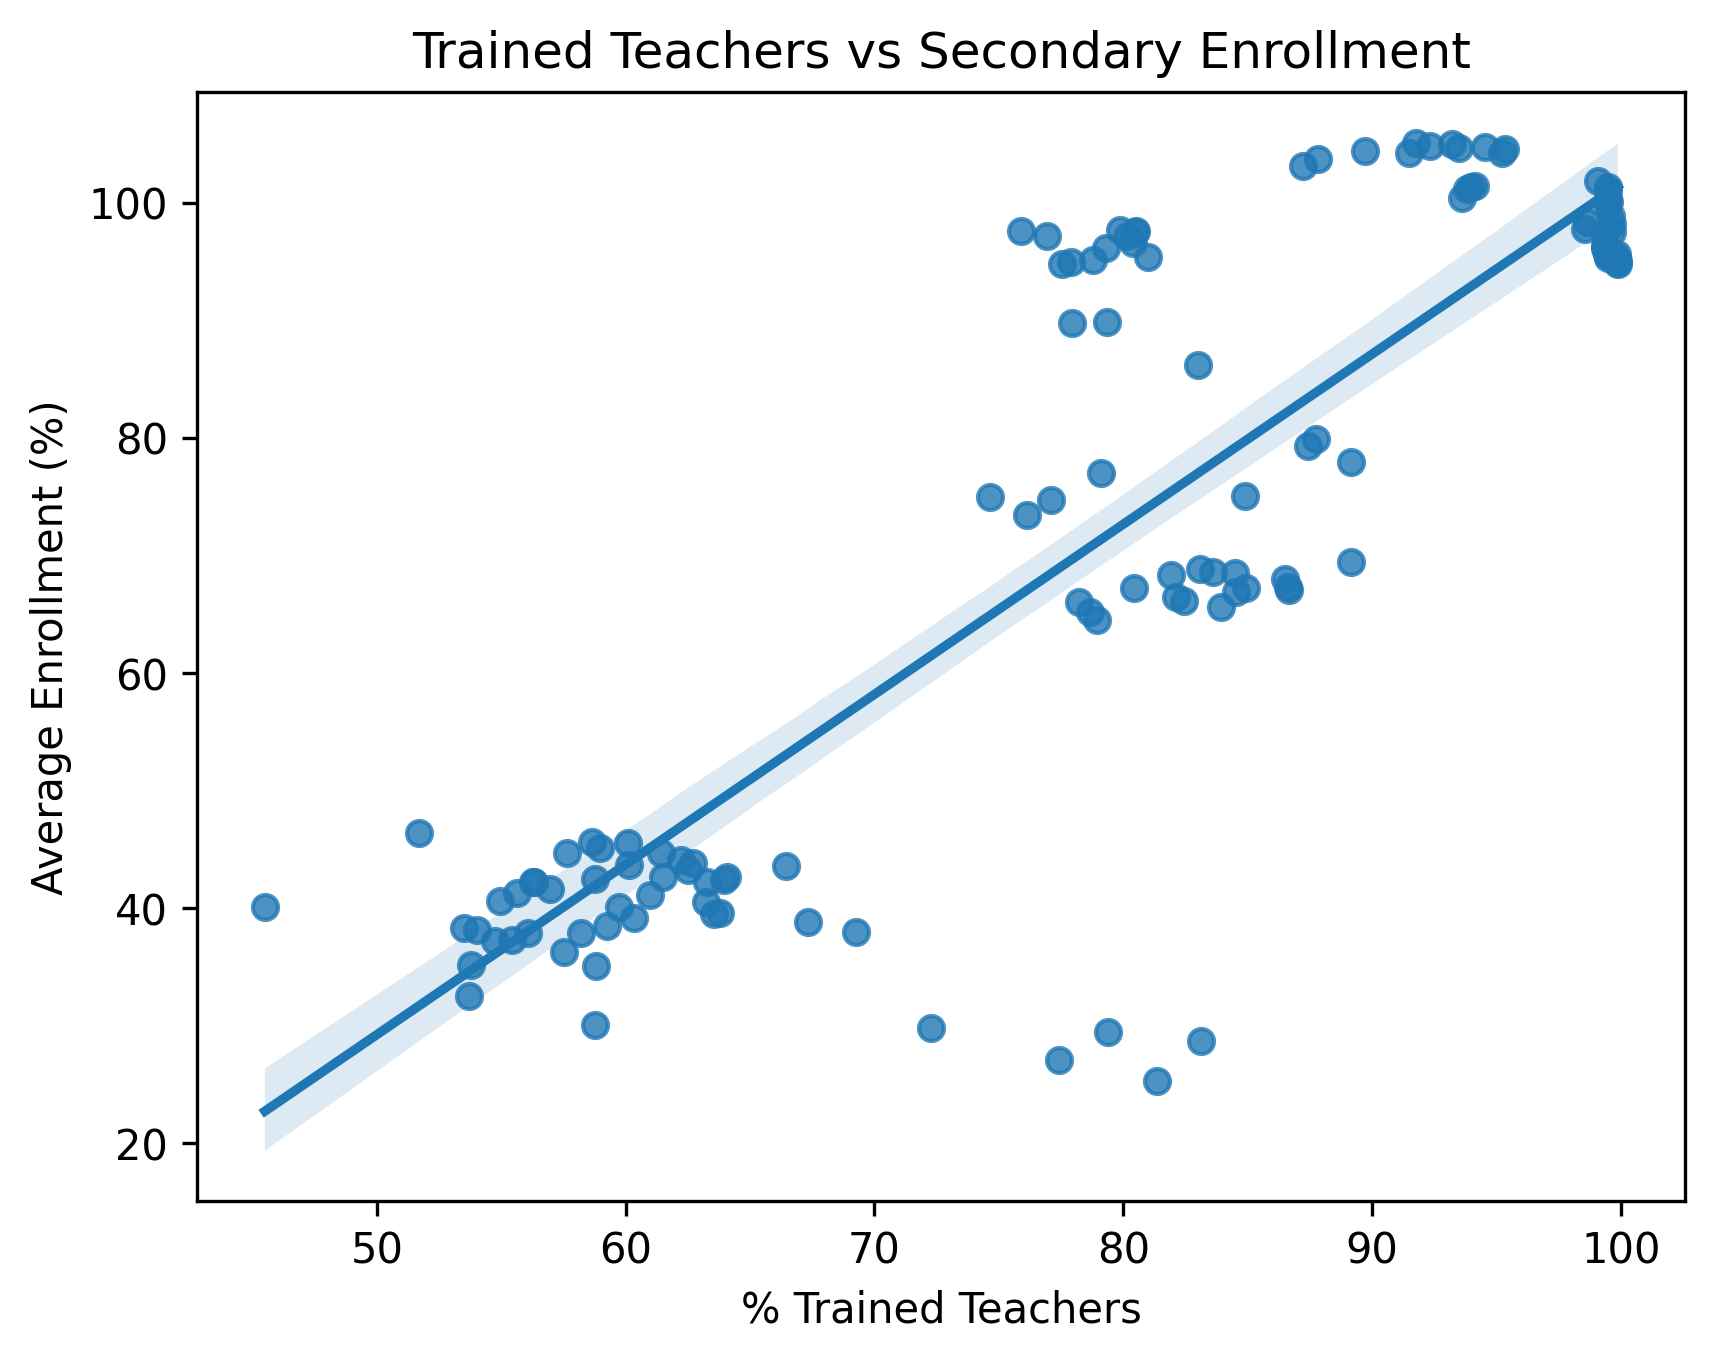
\includegraphics[width=0.65\linewidth,height=\textheight,keepaspectratio]{../figures/teachers_vs_enrollment.png}

}

\caption{Trained teachers vs average secondary enrollment}

\end{figure}%

\subsubsection{Trends Over Time}\label{trends-over-time}

The time-series plot shows that trained teacher percentages and average
secondary enrollment have moved in opposite directions for much of the
study period. Trained teacher percentages started near 100\% in 2000 and
declined to around 75\% by 2010 before partially recovering. Average
secondary enrollment, by contrast, rose steadily from around 61\% in
2000 to approximately 90\% by 2023. The two lines converge around
2010--2012, after which enrollment continues rising while trained
teacher percentages stabilize. This divergence suggests that enrollment
growth has not been driven primarily by increases in teacher training
rates, and that other factors --- such as infrastructure investment,
policy changes, and demographic shifts --- have also contributed.

\begin{figure}[H]

{\centering 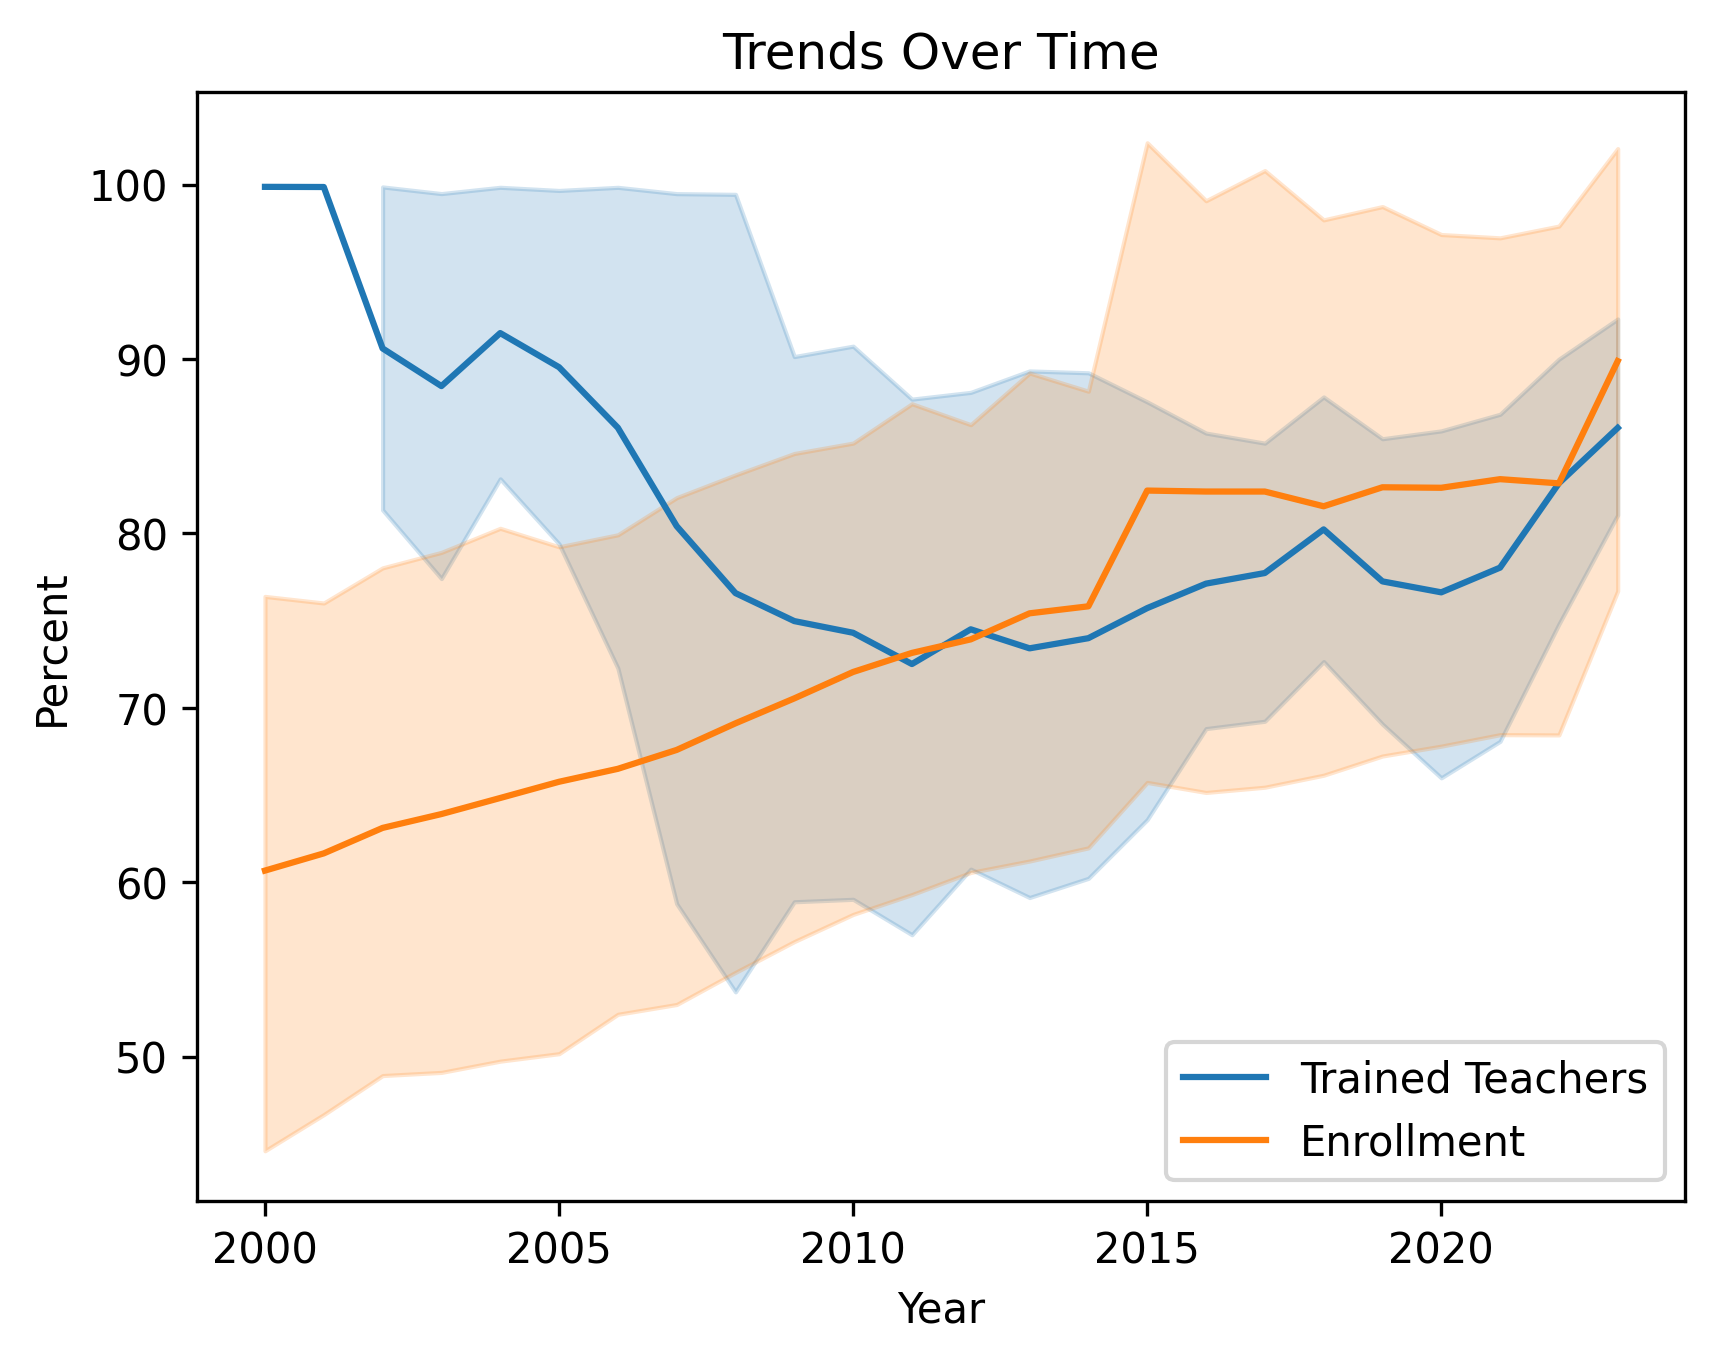
\includegraphics[width=0.65\linewidth,height=\textheight,keepaspectratio]{../figures/time_trends.png}

}

\caption{Trends over time: trained teachers and secondary enrollment}

\end{figure}%

\subsubsection{Gender Comparison}\label{gender-comparison}

When comparing the relationship separately for male and female
enrollment, both show a strong positive association with trained teacher
percentage. The male regression line sits slightly above the female line
at lower trained teacher percentages, suggesting that in regions where a
smaller share of teachers are trained, male enrollment tends to be
somewhat higher than female enrollment. However, the two lines converge
at higher trained teacher percentages, suggesting that as teacher
quality improves, the gender gap in secondary enrollment narrows.

\begin{figure}[H]

{\centering 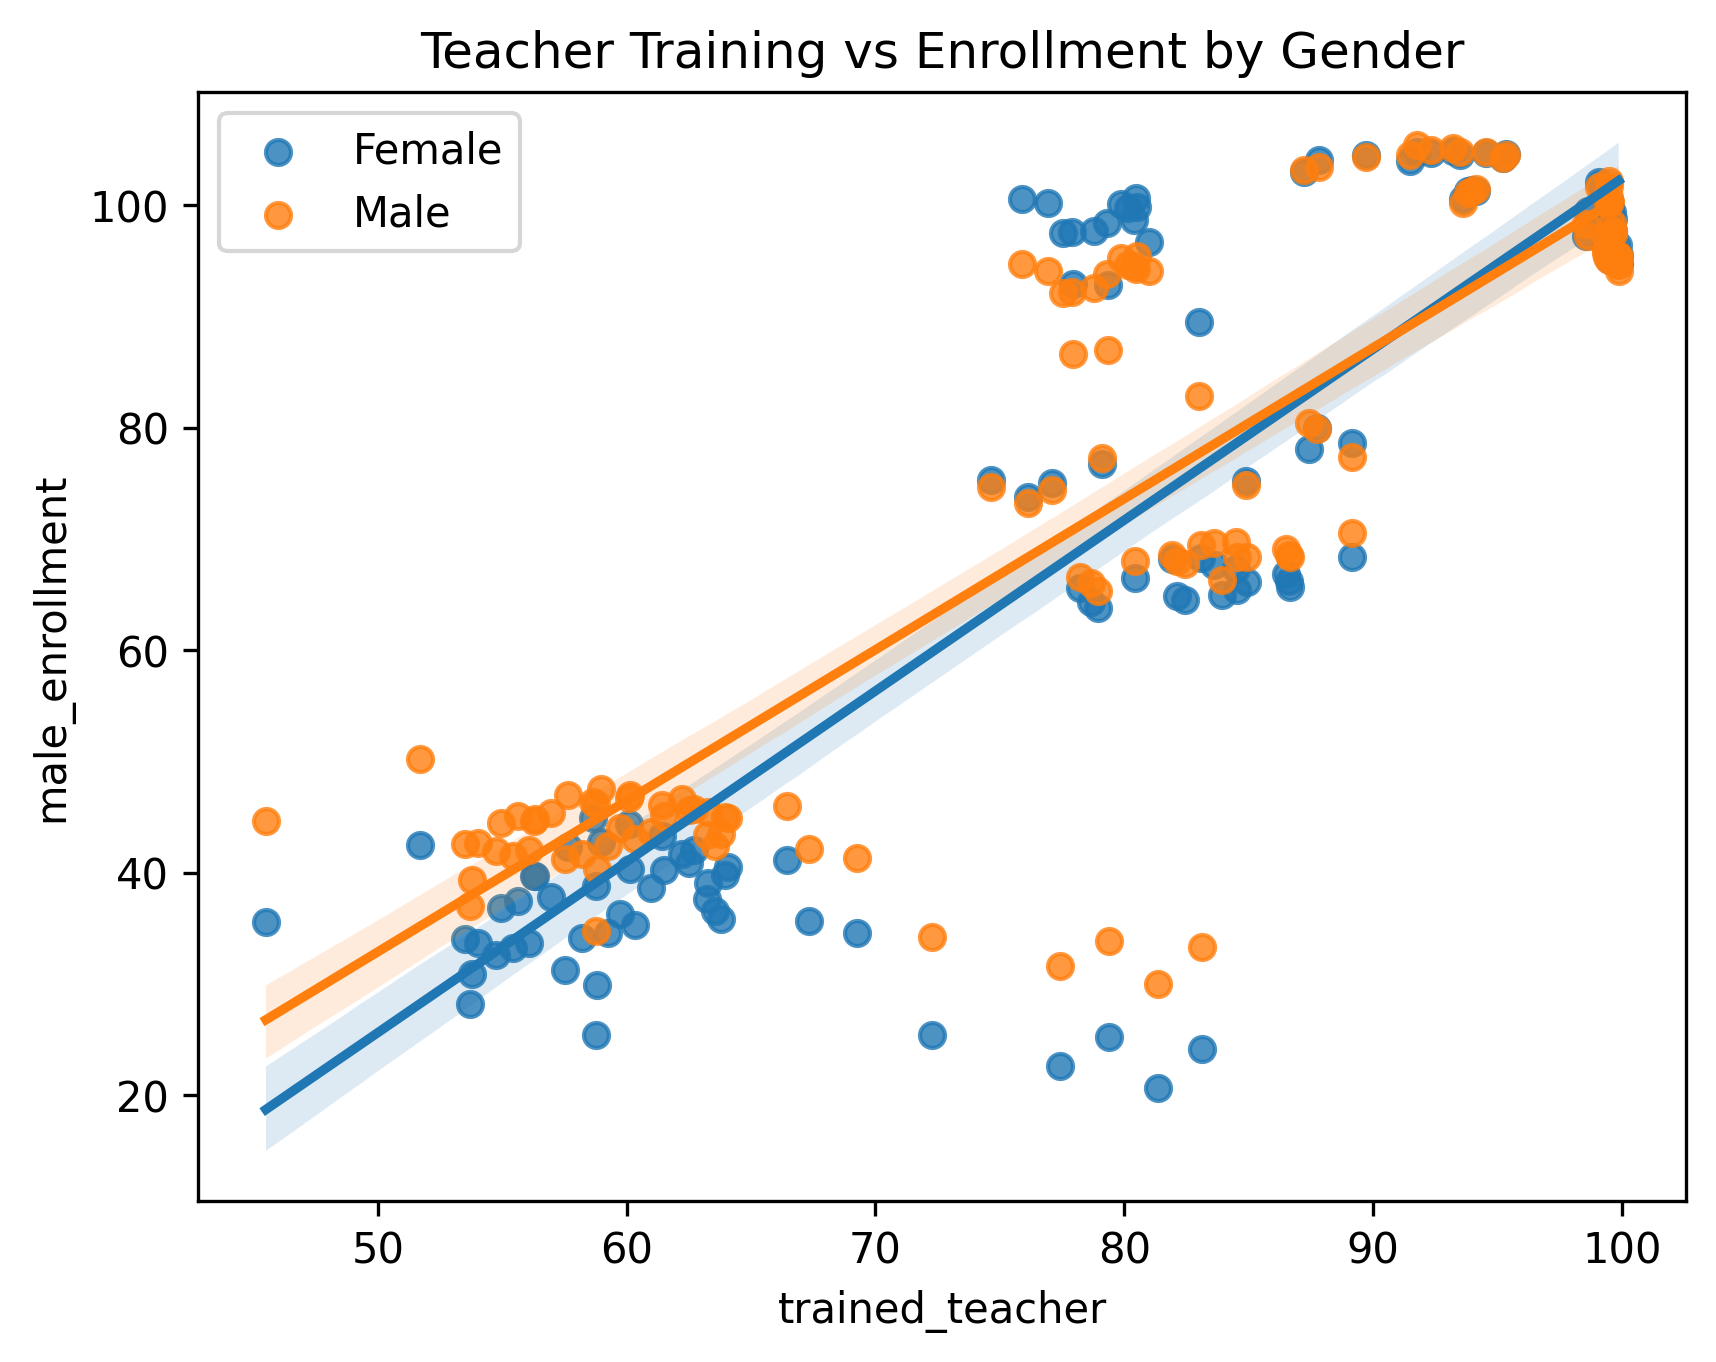
\includegraphics[width=0.65\linewidth,height=\textheight,keepaspectratio]{../figures/gender_comparison.png}

}

\caption{Teacher training vs secondary enrollment by gender}

\end{figure}%

\section{Results and Discussion}\label{results-and-discussion}

Enrollment patterns differ clearly by education level. Primary
enrollment remains near universal for both genders throughout the
period, while secondary enrollment increases steadily over time. The
most substantial gains occur in tertiary education, where enrollment
rises significantly for both males and females, indicating expanded
access to higher education over time.

Gender gaps evolve differently across levels. At the primary and
secondary levels, a small male advantage early in the period steadily
declines, approaching parity in recent years. In contrast, tertiary
education shows a reversal, with female enrollment surpassing male
enrollment and the gap widening over time. This suggests that gender
inequality in education has not disappeared but instead shifted toward
higher levels of education.

Regional disparities further reinforce these patterns. High-income
regions, such as North America, Australia, and the European Union,
exhibit the highest levels of tertiary enrollment, often far exceeding
those in lower-income regions. In contrast, regions such as South Asia
and the Arab World remain substantially behind, highlighting that
overall access to education remains closely tied to economic development
even as gender gaps narrow.

The relationship between teacher training and enrollment is also
positive. Regions with higher proportions of trained teachers tend to
exhibit higher enrollment rates, suggesting that education quality may
support greater participation. However, this relationship should be
interpreted cautiously due to substantial missing data in the teacher
training variable, which limits the strength of any conclusions.

\section{Conclusion}\label{conclusion}

This project analyzed gender disparities in school enrollment and the
relationship between trained teacher percentages and enrollment across
global regions and income groups from 2000 to 2023. We found that gender
gaps in primary and secondary enrollment have narrowed substantially,
while at the tertiary level, female enrollment has consistently exceeded
male enrollment and the gap has widened to nearly -16 percentage points
by 2023. The analysis also found a strong positive association between
trained teacher percentage and secondary enrollment levels, with an R²
of 0.709, and evidence that higher teacher training rates are associated
with a narrowing of the secondary gender gap.

Because trained teacher data is missing for a substantial portion of
region-year observations, the analysis may overrepresent regions with
more complete reporting, limiting the generalizability of these results.
Future work could incorporate country-level data for more granular
insights, or extend the analysis to include additional indicators such
as learning outcomes or government education expenditure. It would also
be valuable to delve into the effects of specific programs designed to
increase enrollment to explore how they can be improved.

\section{Citations}\label{citations}

World Bank. ``Education Statistics --- All Indicators.'' DataBank, World
Bank Group,
https://databank.worldbank.org/source/education-statistics-\%5E-all-indicators.
Wang, Feng, et al.~``An Empirical Analysis of the Impact of Higher
Education on Economic Growth: The Case of China.'' PLOS ONE, 2022,
https://pmc.ncbi.nlm.nih.gov/articles/PMC9435527/. Pholphirul, Piriya.
``Teacher Shortages and Educational Outcomes in Developing Countries:
Empirical Evidence from PISA-Thailand.'' Cogent Education, 2023,
https://www.tandfonline.com/doi/full/10.1080/2331186X.2023.2243126.




\end{document}
